%%%%%%%%%%%%%%%%%%%%%%%%%%%%%% -*- Mode: Latex -*- %%%%%%%%%%%%%%%%%%%%%%%%%%%%
%% dissertation.tex -- 
%% Author          : Carleton Moore
%% Created On      : Mon Oct  5 10:45:35 1998
%% Last Modified By: Carleton Moore
%% Last Modified On: Thu Oct 28 15:03:05 1999
%% RCS: $Id: dissertation.tex,v 1.2 1999/10/19 20:52:32 cmoore Exp cmoore $
%%%%%%%%%%%%%%%%%%%%%%%%%%%%%%%%%%%%%%%%%%%%%%%%%%%%%%%%%%%%%%%%%%%%%%%%%%%%%%%
%%   Copyright (C) 1998 Carleton Moore
%%%%%%%%%%%%%%%%%%%%%%%%%%%%%%%%%%%%%%%%%%%%%%%%%%%%%%%%%%%%%%%%%%%%%%%%%%%%%%%
%% 

%% The options are (you can only choose one from each group):
%%
%% 10pt, 11pt, 12pt: chooses the point size for the document. "11pt" is the
%%                   default.
%%
%% oneside, twoside: whether you want your document onesided or twosided. Note
%%                   that twosided is not guaranteed to work, and style
%%                   guidelines prohibit double sided printouts on final
%%                   copy. "oneside" is the default.
%%
%% draft, final: when printing drafts you can save a lot of paper by using the
%%               "draft" option. It switches to single spacing, displays overful
%%               hboxes with a black box, prints a version number on title page 
%%               and omits signature page. Of course for the final copy make
%%               sure to use the "final" option! "final" is the default.
%%
%% cm, times, palatino, newcent, bookman: switches between different font
%%                                        sets. "cm" is the Computer Modern
%%                                        font (TeX's default), the rest are
%%                                        PostScript fonts. "times" is the
%%                                        default.
%%
%% thesis, dissertation: switches between the style for a master's thesis and a 
%%                       Ph.D. dissertation. The differences are fairly minor
%%                       and limited to the front matter. "thesis" is the
%%                       default.
%%
%% actual, proposal: switches between actual document and proposal mode. In
%%                   proposal mode: the title page is simplified, the
%%                   version number is always printed, and the signature page
%%                   is omitted.
%%
%%% Load the uhthesis2e document class
\documentclass[11pt,times,dissertation,proposal]{uhthesis2e}
%\documentclass[11pt,times,dissertation]{uhthesis2e}

%%% Load some useful packages:
%% New LaTeX2e graphics support
\usepackage{graphicx}
%% Package to linebreak URLs in a sane manner.
\usepackage{url}
\usepackage{shapepar}

%%% End of preamble
\begin{document}

%%% Declarations for Front Matter. Capitalize all of these values
%%% "normally". This allows the document class to format them properly.
%% Full title of thesis or dissertation, capitalized like a title should be.
\title{Automated Support for Technical Skill Acquisition and Improvement: An
Evaluation of the Leap Toolkit}
%% Your name, capitalized normally. Do not include any titles like Dr.
\author{Carleton A. Moore}
%% Month in which you intend to receive your degree (i.e. graduation).
%% Presumably this will be one of: May, August, or December.
\degreemonth{May}
%% Year of expected graduation.
\degreeyear{2000}
%% Type of degree to be conferred.
\degree{Doctor of Philosophy}
%% This is the chairperson of your committee. Do not use titles like Dr.
\chair{Philip Johnson}
%% The other members of your committee, seperated by "\\". Again, no titles,
%% and it is customary to list the outside committee member (if you have one)
%% last.
\othermembers{James Corbett\\
  Elizabeth Davidson \\
  Marie Iding \\
  Larry Osborne}
%% This is the total size of your committee, including the chairperson. The
%% signature page routine will only handle up to 6 members; if you have more
%% than that you will need to modify the document class.
\numberofmembers{5}
%% The field in which you are obtaining your degree, capitalized normally.
\field{Communication and Information Sciences}
%% The version number of your document. Consistent use of this will enable you
%% to tell old drafts from new ones. Final actual documents omit this
%% automatically so you can use it without fear of submission problems at the
%% end. If you do not define this parameter, it defaults to "1.0.0".
\versionnum{2.0.3}

\setcounter{tocdepth}{6}
\setcounter{secnumdepth}{10}
%%% Create the title page from all the information above. Note that the
%%% titlepage is outside the front matter.
\maketitle

\begin{frontmatter}

%%% Create the signature page (when indicated by the options)
\signaturepage

%%% Create the copyright page
%\copyrightpage

%%% Bring in the dedication page from external file
%%%%%%%%%%%%%%%%%%%%%%%%%%%%%%% -*- Mode: Latex -*- %%%%%%%%%%%%%%%%%%%%%%%%%%%%
%% diss-dedication.tex -- 
%% Author          : Carleton Moore
%% Created On      : Mon Oct  5 10:52:13 1998
%% Last Modified By: Carleton Moore
%% Last Modified On: Mon Oct  5 10:54:07 1998
%% RCS: $Id: diss-dedication.tex,v 1.1 1998/10/05 20:54:25 cmoore Exp $
%%%%%%%%%%%%%%%%%%%%%%%%%%%%%%%%%%%%%%%%%%%%%%%%%%%%%%%%%%%%%%%%%%%%%%%%%%%%%%%
%%   Copyright (C) 1998 Carleton Moore
%%%%%%%%%%%%%%%%%%%%%%%%%%%%%%%%%%%%%%%%%%%%%%%%%%%%%%%%%%%%%%%%%%%%%%%%%%%%%%%
%% 

\begin{dedication}\null\vfil
{\large
\begin{center}
To \\\vspace{12pt}
My parents\\\vspace{12pt}
and CSDL\\\vspace{12pt}
\end{center}}
\vfil\null
\end{dedication}


%%% Bring in the acknowledgements section from external file
%%%%%%%%%%%%%%%%%%%%%%%%%%%%%%% -*- Mode: Latex -*- %%%%%%%%%%%%%%%%%%%%%%%%%%%%
%% diss-acknowledgements.tex -- 
%% Author          : Carleton Moore
%% Created On      : Mon Oct  5 10:54:56 1998
%% Last Modified By: Carleton Moore
%% Last Modified On: Mon Oct  5 10:56:46 1998
%% RCS: $Id: diss-acknowledgements.tex,v 1.1 1998/10/05 20:56:57 cmoore Exp $
%%%%%%%%%%%%%%%%%%%%%%%%%%%%%%%%%%%%%%%%%%%%%%%%%%%%%%%%%%%%%%%%%%%%%%%%%%%%%%%
%%   Copyright (C) 1998 Carleton Moore
%%%%%%%%%%%%%%%%%%%%%%%%%%%%%%%%%%%%%%%%%%%%%%%%%%%%%%%%%%%%%%%%%%%%%%%%%%%%%%%
%% 

\begin{acknowledgements}

CIS Students

CSDL

Mom and Dad

Scott

\end{acknowledgements}

%%% Bring in the abstract section from external file
%%%%%%%%%%%%%%%%%%%%%%%%%%%%%% -*- Mode: Latex -*- %%%%%%%%%%%%%%%%%%%%%%%%%%%%
%% diss-abstract.tex -- 
%% Author          : Carleton Moore
%% Created On      : Mon Oct  5 10:57:35 1998
%% Last Modified By: Carleton Moore
%% Last Modified On: Wed Oct 27 08:02:08 1999
%% RCS: $Id: diss-abstract.tex,v 1.2 1999/10/27 20:31:14 cmoore Exp $
%%%%%%%%%%%%%%%%%%%%%%%%%%%%%%%%%%%%%%%%%%%%%%%%%%%%%%%%%%%%%%%%%%%%%%%%%%%%%%%
%%   Copyright (C) 1998 Carleton Moore
%%%%%%%%%%%%%%%%%%%%%%%%%%%%%%%%%%%%%%%%%%%%%%%%%%%%%%%%%%%%%%%%%%%%%%%%%%%%%%%
%% 

\begin{abstract}
  Software developers work too hard and yet do not get enough done.  Developing
  high quality software efficiently and consistently is a very difficult
  problem.  Developers and managers have tried many different solutions to
  address this problem.  Recently their focus has shifted from the software
  organization to the individual software developer.  The Personal Software
  Process incorporates many of the previous solutions while focusing on the
  individual software developer.
  
  I combined ideas from prior research on the Personal Software Process, Formal
  Technical Review and my experiences building automated support for software
  engineering activities to produce the Leap toolkit.  The Leap toolkit is
  intended to help individuals in their efforts to improve their development
  capabilities.  Since it is a light-weight, flexible, powerful, and private
  tool, it allows individual developers to gain valuable insight into their own
  development process. The Leap toolkit also addresses many measurement and
  data issues involved with recording any software development process.
  
  The main thesis of this work is the Leap toolkit provides a more accurate and
  effective way for developers to collect and analyze their software
  engineering data than manual methods.  To evaluate this thesis I will
  investigate three claims: (1) the Leap toolkit prevents many important errors
  in data collection and analysis; (2) the Leap toolkit supports data
  collection and analyses that are not amenable to manual enactment; and (3)
  the Leap toolkit reduces the level of ``collection stage'' errors.  To
  evaluate the first claim, I will show how the design of the Leap toolkit
  effectively prevents important classes of errors shown to occur in prior
  related research. To evaluate the second claim, I will conduct an experiment
  investigating 14 different quantitative time estimation techniques based upon
  historical size data to show that the Leap toolkit is capable of complex
  analyses not possible in manual methods.  To evaluate the third claim, I will
  analyze software developers data and conduct surveys to investigate the level
  of data collection errors.
  
%  This research will show that the Leap toolkit is an effect tool for
%  individual software developer improvement.

\end{abstract}


%%% Generate table of contents
\tableofcontents

%%% Generate list of tables
\listoftables

%%% Generate list of figures
\listoffigures

\end{frontmatter}

%%% Bring in the body of the thesis from external file
%%%%%%%%%%%%%%%%%%%%%%%%%%%%%% -*- Mode: Latex -*- %%%%%%%%%%%%%%%%%%%%%%%%%%%%
%% diss-intro.tex -- 
%% Author          : Carleton Moore
%% Created On      : Mon Oct  5 10:58:59 1998
%% Last Modified By: Carleton Moore
%% Last Modified On: Wed Oct 27 10:30:51 1999
%% RCS: $Id: diss-intro.tex,v 1.4 1999/10/27 20:30:54 cmoore Exp $
%%%%%%%%%%%%%%%%%%%%%%%%%%%%%%%%%%%%%%%%%%%%%%%%%%%%%%%%%%%%%%%%%%%%%%%%%%%%%%%
%%   Copyright (C) 1998 Carleton Moore
%%%%%%%%%%%%%%%%%%%%%%%%%%%%%%%%%%%%%%%%%%%%%%%%%%%%%%%%%%%%%%%%%%%%%%%%%%%%%%%
%% 

\chapter{Introduction}
\label{sec:intro}
\begin{quote}
{\em At the start, when we know much about the problem and nothing about the
solution, the solution is very abstract.} -- Robert H. Dunn
\end{quote}

Every software developer wishes they got home from work sooner and spent less
of their weekend at work. Software developers work very hard and very long, yet
software is often delivered late, over budget, and full of defects.  Over forty
years of software development experience has not helped us solve this problem.
How can software developers gain more control over their software development
and produce high quality software efficiently?  Project LEAP and the Leap
toolkit in particular attempts to give developers the control and skills they
need.  Before I discuss Leap I will give a short background of the software
development problem.

\section{Why is Quality Software Development Important?}



Software is controlling more safety critical tasks and important
functions\cite{Armour93}. Yet software errors occur sometimes with horrible
costs. Between 1985 and 1987 the Therac-25 radiation therapy machine killed two
people and seriously injured four others by delivering massive radiation
overdoses.  Investigations found that many issues were to blame including
faulty software\cite{Leveson93}.

In March 1995, the Denver International Airport opened over 16 months late and
over 100 million dollars over budget. One of the primary reasons for the delay
and overrun was the presence of major bugs in the baggage handling control
software\cite{Glass98}.

Another problem with current software development is productivity. The
insatiable demand for more software has out-paced our ability to produce
software.  Software productivity has not kept pace with hardware
cost/performance ratios. The most optimistic rate at which programmer
productivity is increasing is 5\% per year, while there is greater than a ten
fold increase in the demand for software each decade.\cite{Dunn90} The
government of the United States of America faces this problem. In 1996
Computerworld reported that delays in overhauling the federal tax computer
systems cost the U.S.  Treasury as much as \$50 billion per year.\cite{Glass98}
The problem of overhauling of the tax computers is not purely a software issue
but the software system is a large part of the problem.

\section{Traditional Solutions}

Software developers and managers have addressed software quality and
development issues since the beginning of the computer age. Developer and
managers have continuously augmented the development methods they use. We can
divide these methods into four eras: hope-based, product-based,
organization-based, and individual-based.  Figure \ref{fig:eras} shows a time
line of software development improvement and the different eras.

\begin{center}
  \begin{figure}[htb]
    \setlength{\unitlength}{2.5cm}
    \begin{picture}(6,3)
      \setlength{\fboxsep}{0.25cm}
      \thicklines
      \put(0.25,1.5){\vector(1,0){5.5}}
      \thinlines
      \put(5.6,1.6){Time}
      \put(1,1.5){\circle*{0.15}}
      \put(1.3,1.6){1960s}
      \put(2,1.5){\circle*{0.15}}
      \put(2.3,1.3){1970s}
      \put(3,1.5){\circle*{0.15}}
      \put(3.3,1.6){1980s}
      \put(4,1.5){\circle*{0.15}}
      \put(4.3,1.3){1990s}
      \put(5,1.5){\circle*{0.15}}
      \put(0.9,0.25){\framebox(1.25,0.5){\parbox[b]{2.5cm}{Hope-based (Try
            harder)}}}
      \put(1.2,0.8){\begin{picture}(0.75, 0.75)
          \put(0.25,0){\line(0,1){0.3}}
          \put(0.5,0){\line(0,1){0.3}}
          \put(0.05,0.3){\line(1,0){0.2}}
          \put(0.7,0.3){\line(-1,0){0.2}}
          \put(0.05,0.3){\line(1,1){0.32}}
          \put(0.7,0.3){\line(-1,1){0.32}}
        \end{picture}}
      \put(1.9,2.5){\fbox{\parbox[b]{2.5cm}{Product-based (Testing, FTR)}}}
      \put(2.2,1.5){\begin{picture}(0.75, 0.75)
          \put(0.25,0.75){\line(0,-1){0.3}}
          \put(0.5,0.75){\line(0,-1){0.3}}
          \put(0.05,0.45){\line(1,0){0.2}}
          \put(0.7,0.45){\line(-1,0){0.2}}
          \put(0.05,0.45){\line(1,-1){0.32}}
          \put(0.7,0.45){\line(-1,-1){0.32}}
        \end{picture}}
      \put(2.7,0.25){\fbox{\parbox[b]{3.5cm}{Organizational-based
            (CMM, ISO 9000)}}}
      \put(3.2,0.8){\begin{picture}(0.75, 0.75)
          \put(0.25,0){\line(0,1){0.3}}
          \put(0.5,0){\line(0,1){0.3}}
          \put(0.05,0.3){\line(1,0){0.2}}
          \put(0.7,0.3){\line(-1,0){0.2}}
          \put(0.05,0.3){\line(1,1){0.32}}
          \put(0.7,0.3){\line(-1,1){0.32}}
        \end{picture}}
      \put(3.9,2.5){\fbox{\parbox[b]{3cm}{Individual-based
            (PSP)}}}
      \put(4.2,1.5){\begin{picture}(0.75, 0.75)
          \put(0.25,0.75){\line(0,-1){0.3}}
          \put(0.5,0.75){\line(0,-1){0.3}}
          \put(0.05,0.45){\line(1,0){0.2}}
          \put(0.7,0.45){\line(-1,0){0.2}}
          \put(0.05,0.45){\line(1,-1){0.32}}
          \put(0.7,0.45){\line(-1,-1){0.32}}
        \end{picture}}      
    \end{picture}
    \caption{Eras of Software Development Improvement}
    \label{fig:eras}
  \end{figure}
\end{center}

In the 1960's much of the software development improvement efforts were just
focused on doing better. The problems of software development tended to be
small since computers were very small as compared to today's computers.  Trying
harder seemed like a reasonable solution.  

%The water-fall development model was
%introduced.

In the 1970's people realized while the ``try-harder'' method did help improve
software development it was not enough. Computers and software programs were
getting more complex and new methods were needed. Developers and researchers
started looking at the work products. Many Developers and Computer Scientists
advocated testing to help improve the quality of software. In 1976 Fagan
reported on Software Inspection's\cite{Fagan76} success as a method to
efficiently improve the quality of the work product.  

In the late 1980's the focus shifted from the work products to the
organizations that produced the work products. The SEI introduced the Capability
Maturity Model\cite{Paulk95} and ISO 9000\cite{ISO9000} became wide spread.  These
organizational processes helped improve software quality and the development
processes but didn't completely solve the problem.

In the late 1990's some Computer Scientists and Developers changed their focus
again from the organization to the individual software developer. In 1995
Humphrey introduced the Personal Software Process\cite{Humphrey95}, a software
development process and improvement process for individual software developers.
The PSP is a manual process where the developer collects data about the amount
of time they spend, the size of the work product and the defects they make
while developing software.  By analyzing the data at the end of the project,
the developer gains insights into their development process.  These insights
help the developer increase productivity and work product quality.

%In the past four years, there has arisen a new focus on the individual
%software developer.  One such effort is Watts Humphrey's Personal Software
%Process, PSP\cite{Humphrey95}.  In PSP, software engineers record the time
%they spend programming, the defects they find in their software and the
%size of the software.  Based upon these measurements, engineers can
%track their productivity, make better predictions for future projects, gain
%insight to what types of errors they make, and learn how to remove defects
%earlier in their development process.  The PSP, as described by Humphrey,
%is a completely manual process. 

Many studies have shown the PSP helps improve software
development\cite{Ferguson97,Hayes97,Khajenoori95,Ramsey96}, but is not the
complete solution to the software development issue. 

After using the PSP for two years in our research group, the Collaborative
Software Development Laboratory (CSDL), we decided to try to build upon the PSP's
strong foundation and incorporate features of formal technical review to
produce a more effective software developer improvement tool.

\section{LEAP: Giving developers more control and insight}

LEAP is a design philosophy intended to produce effective tools that allow
developers to gain valuable insight into their own software development.  Using 
the LEAP design philosophy I developed the Leap toolkit, a Java application
that supports technical skill acquisition.

\subsection*{Using the Leap toolkit example}
I will introduce the Leap toolkit by using a hypothetical software developer,
Cam, and his manager, Philip. Cam and Philip work for a small world class Java
software development company.  Cam has been using the Leap toolkit for about a
year to keep track of his Java programming projects.  He has a small database
of over 30 Java projects.  

\subsubsection*{Starting a new project} 
Philip calls Cam into his office to discuss Cam's next project.  The next
project is an extension to their single user calendar tool that allows multiple
users to use the same calendar while keeping some events private.  Philip gives
Cam the requirements for the new extension and ask him how long the project
will take.  Cam tells Philip that he needs to do some design work before he can
give an accurate estimate.  Cam goes back to his cubicle and starts the Leap
toolkit shown in Figure \ref{fig:LeapController}.
\begin{figure}[p]
  \centering
  \includegraphics[angle=270,bb=195 280 250 510]{LeapController.eps}
  \caption{Leap Toolkit Controller. This is the main controller for the Leap
  toolkit. The developer may start data recording tools or start tools to
  modify their definitions.}
  \label{fig:LeapController}
\end{figure}

\subsubsection*{Defining the new project}
To start the new project Cam opens the Projects (Ilio) tool.  To create a new
project Cam starts the project editing tool Hee on the first blank line. He
types in the name of the new project ``Multi-User Calendar'' and a brief
description of the project.  Then he selects the start date for the project and 
chooses the PhaseSet that he plans on using.  The PhaseSet is a set of phases
that describe his development process.  Cam evolved his current PhaseSet after
experimenting with different development processes.  Figure \ref{fig:hee-start} shows
the Hee project viewer.
\begin{figure}[p]
  \centering
  \includegraphics[angle=270,width=6in,bb=45 130 600 665]{hee-main.ps}
  \caption{Hee Project Viewer.  This tool allows the developer to define, plan
  and analyze a single project. Cam has filled out the name, description and
  start date for the Multi-User Calendar project.  He has also decided to use his
  Development process for this project.}
  \label{fig:hee-start}
\end{figure}

\subsubsection*{Developing an initial design}
Cam then starts the Io timer tool to record the time he spends designing the
new project. Figure \ref{fig:io-start} shows the Io timer after he started
recording time for the design phase.
\begin{figure}[p]
  \centering
  \includegraphics[angle=270,width=5in]{io-start.ps}
  \caption{Io time recording tool. Io allows the developer to easily record the 
  amount of time they spend working on a task.  They may also account for any
  interruptions by recording interrupt time. In this Figure Cam has worked for
  40 minutes on the design of the Multi-User Calendar.}
  \label{fig:io-start}
\end{figure}

Cam works on the design for the new project and when he finishes his design he
clicks the stop button on Io and then records his time in the Leap toolkit.

\subsubsection*{Project Planning}
With the initial design of 30 classes and 168 methods. 
\paragraph*{Size Planning}
Cam then opens the Project Comparisons tool to find out his average lines of
code per method. His average is 17.99 lines of code per method so he calculates
that the whole project will be 3022 lines of code.  He reopens the Hee project
viewer for the Multi-User calendar project and enters in his planned sizes.
\paragraph*{Estimating effort}
He then goes to the time tab in Hee and starts the time estimation tool. Cam
choose to use his historical average rates for the trend lines and lines of
code for the size grain size then presses the estimate button. Figure
\ref{fig:timeest1} shows the time estimation tool with the estimate.  Based
upon his historical data this project will take about 2010 minutes.  Cam tries
some of the other combinations like methods and linear regression model to give
him a range of estimates.  Based upon all these estimates, Cam estimates that
it will take him anywhere from 28 1/3 hours to 38 2/3 hours of direct work to
complete the project. Cam enters in his time estimate into Hee and then sets up
a meeting with Philip.
\begin{figure}[htbp]
  \centering
  \includegraphics[angle=270,width=6in,bb=67 58 546 734]{timeest1.ps}
  \caption{Time Estimation Tool. The time estimation tool shows Cam's
    historical data.  Cam has chosen Linear Regression for the trend lines and
    Lines of code as the size measures for time estimation. The planned size
    3022 is taken from Hee.  Based upon this data the project should take from
    1699 to 2321 minutes.}
  \label{fig:timeest1}
\end{figure}

\subsubsection*{Negotiation}
At the meeting with Philip, Cam tells Philip that the project will take him
between two and three weeks.  From Cam's historical data he knows that he only
gets in an average of 3 direct hours per project per work day so the 28 1/3
direct hours will take 9 1/2 days to complete. Philip wants the project done in 
one week.  Cam says that this is only possible if he can stop working on his
other projects and focus solely on the Multi-User Calendar project.  Philip
agrees that Cam may drop his other projects until the calendar is finished.


\section{Thesis Statement}

LEAP provides a more accurate and effective way for developers to collect and
analyze their software engineering data than methods designed for manual
enactment. 

\section{Evaluation of the Leap toolkit}

I will evaluate the main thesis of this work by breaking the thesis down into
three claims. 

First, the Leap toolkit prevents many important errors. To evaluate this claim
I will discuss the design and automation features in the Leap toolkit that 
prevent these errors from occurring. 

Second, the Leap toolkit provides data analysis that is not practical with a
manual method. To evaluate this claim I will conduct an empirical experiment to 
determine if any particular time estimation technique is more accurate. Using
the Leap toolkit I will compare 13 different time estimation techniques and
determine if any of them are more accurate in predicting the effort for a new
project. In a manual method, such as the PSP, only one time estimation method
can be provided.

Third, The Leap toolkit reduces the level of collection stage errors. To
evaluate this claim I will conduct four surveys and analyze the software
development data collected by graduate students in an advanced software
engineering course at the University of Hawaii.

\section{Anticipated Contributions}

This research is designed to produce several valuable contributions to the
software engineering community.  One major contribution is the Leap toolkit.  I
have made the Leap toolkit freely available on the Internet.  Software
developers may down-load the Leap toolkit and use it in their own work.  The
Leap toolkit has been available for over one year and many developers have
down-loaded it.  The Leap toolkit also provides a novel tool for software
developer education, as is being demonstrated in a graduate level class in
software engineering this semester.  Instructors can gain insight into how the
students are actually spending their time and provide more detailed help.

Another anticipated contribution is the results of the time estimation
experiment.  The results may indicate that one estimation technique is more
accurate, or that different techniques are more accurate for different people,
or that no technique is significantly better than any other. If it turns out
that there is no more accurate estimation technique then developers can use
simple averages which are easy to calculate instead of complex formulas. If
there is a best estimation technique then developers can adopt it and gain more
accurate time estimations.

\section{Organization of the Proposal}


This proposal is organized as following: Chapter \ref{sec:related} relates the
current research to the broader context of existing work. Chapter
\ref{sec:LEAP} depicts the main design features and planned benefits of LEAP.
Chapter \ref{sec:evaluation} outlines the evaluation methods I plan to use to
evaluate the effectiveness of LEAP.  Finally, Chapter \ref{sec:plan} presents
the current research plan.








%Software developers and managers have faced the problem of producing
%quality software since the beginning of the computer age.  Many people have
%studied the software quality problem and have proposed many solutions.  We
%can categorize these different solutions into two groups: (1) ``Top-down''
%solutions, that focus on software development as a group effort and (2)
%``Bottom-up'' solutions, that focus on the individual software developer.  Some
%of the many Top-down solutions include: the Capability Maturity Model,
%Clean Room development, software quality assurance groups, and Formal
%Technical Review.  These top down methods help improve the quality of the
%software, however they may not be enough. 

%In the past four years, there has arisen a new focus on the individual
%software developer.  One such effort is Watts Humphrey's Personal Software
%Process, PSP\cite{Humphrey95}.  In PSP, software engineers record the time
%they spend programming, the defects they find in their software and the
%size of the software.  Based upon these measurements, engineers can
%track their productivity, make better predictions for future projects, gain
%insight to what types of errors they make, and learn how to remove defects
%earlier in their development process.  The PSP, as described by Humphrey,
%is a completely manual process. 

%After two years of experience with the PSP, we noticed three general
%problems.  First, we started to question the quality of the data recorded.
%For example, we noticed that it is extremely difficult to accurately record
%every defect made during software development, in part because of the
%overhead of collection.  Anne Disney and Philip Johnson conducted a study
%to look at the data quality of PSP data.  They found that there are
%significant data quality issues with manual PSP.\cite{csdl-98-04, csdl-98-05} 

%Second, our experiences with industrial partners, management practices, and
%Robert Austin's book ``Measuring and Managing Performance in
%Organizations''\cite{Austin96} made us think about the issues of
%measurement dysfunction in PSP and review data.  There are many subtle
%pressures on professionals to provide management with ``good'' results.
%While the PSP is a private process, we question whether management directed
%PSP training might not induce measurement dysfunction. 

%Third, after four years, the results with long term adoption of PSP are
%mixed.  Pat Ferguson and others report excellent results with PSP adoption
%at Advanced Information Services, Motorola and Union Switch and
%Signal\cite{Ferguson97}.  However, Barry Shostak and others report poor
%adoption of PSP in industry \cite{Shostak96, Emam96}. 

%These issues started us thinking about how to design an automated,
%empirically based, personal process improvement tool to address these
%issues.  Our goals are to reduce the collection and analysis overhead for
%the engineer, to reduce the potential for measurement dysfunction in the
%collection process, and to allow the engineer to use their own development
%style.  We are also incorporating collaborative review support into our
%personal process improvement tool.  Adding review support allows the
%developer to gain insight from other developers.  This group input is an
%important feature lacking in the PSP.  These features are intended to
%improve the benefits to the engineer and the long term adoption of
%empirically based process improvement.  To pursue this work, we initiated
%Project LEAP, \url{http://csdl.ics.hawaii.edu/Research/LEAP/LEAP.html}, and
%began developing the Leap Tool Set as a ``reference implementation'' of
%these design goals. 

%\section{Research Questions}
%We intend to deploy the Leap Tool Set in both academic and industry
%settings in order to investigate the following research questions:
%\begin{itemize}

%\item{Is the integration of collaborative review and personal data
%    collection appropriate?}
  
%\item{Is Leap an appropriate form of automated support for personal process
%    improvement?}
  
%\item{What are the strengths and weaknesses of the Leap Tool Set and
%    empirically based process improvement?}

%\item{What are the barriers to adoption of the Leap Tool Set?}
  
%\item{What are the benefits to the users of Leap?}

%\item{How do users improve after using Leap and what are the kinds of
%    improvements we can make using Leap?}

%\item{Does the automated data analysis in Leap allow users to change the way
%        they work?}
%\end{itemize}

%One major claim of the PSP is "it makes routine elements of your job more
%predictable" (p. 1, Humphrey95).  For planning the development time for
%small programs the PSP developer follows a flow chart to decide which
%estimation practice to use.  If the developer does not have enough data for 
%a regression calculation or their data is not highly correlated they use
%historical averages.  If they don't have enough time predictions or the
%predictions are not correlated to the actual development times then they
%use regression calculations on the actual sizes and time.  Finally, if the
%developer has enough predictions and they are correlated they use
%regression calculations on the predicted values.  After using this
%procedure and looking at our data we started to ask why is it better to use
%linear regression on our data than historical averages?  Since Leap
%automates much of the analysis of our data we can investigate this issue.

%\section{Hypotheses}
%\begin{enumerate}

%\item {There is no difference in accuracy between using historical averages and linear
%regression in making predictions.}
  
%\item {Given multiple methods of predictions developers will use an
%intermediate value for their prediction.}
  
%\item {The user's predictions will be more accurate than the pure historical
%prediction or linear regression prediction.}
  

%\end{enumerate}



 %Introduction
%%%%%%%%%%%%%%%%%%%%%%%%%%%%%% -*- Mode: Latex -*- %%%%%%%%%%%%%%%%%%%%%%%%%%%%
%% diss-related.tex -- 
%% Author          : Carleton Moore
%% Created On      : Thu Sep  2 11:02:52 1999
%% Last Modified By: Carleton Moore
%% Last Modified On: Wed Oct 27 10:29:35 1999
%% RCS: $Id: diss-related.tex,v 1.3 1999/10/27 20:29:41 cmoore Exp $
%%%%%%%%%%%%%%%%%%%%%%%%%%%%%%%%%%%%%%%%%%%%%%%%%%%%%%%%%%%%%%%%%%%%%%%%%%%%%%%
%%   Copyright (C) 1999 Carleton Moore
%%%%%%%%%%%%%%%%%%%%%%%%%%%%%%%%%%%%%%%%%%%%%%%%%%%%%%%%%%%%%%%%%%%%%%%%%%%%%%%
%% 

\chapter{Related Work}
\label{sec:related}

\begin{quote}
{\em If you don't know what you are doing, it is hard to improve it.} -- Watts Humphrey
\end{quote}

LEAP is a result of our experience using the Personal Software Process (PSP)
for over three years, our experience with Formal Technical Review (FTR) and our
attempts to improve the quality of software development.  This chapter briefly
discusses the PSP, some of the different tools developed to support the PSP,
and the software quality assurance process called Formal Technical Review.  The
chapter concludes with a discussion of measurement dysfunction and some of the
data quality issues found in the PSP and FTR.

\section{Personal Software Process}

The Personal Software Process\cite{Humphrey95} is a self-improvement process
for software developers. In his book ``A Discipline for Software Engineering''
Watts Humphrey teaches software developers how to become their own software
development coaches. Sports coaches observe the performance of their players,
evaluate their performance, then make suggestions for improvement.  This is the
classic {\em observe, evaluate, modify} cycle for improvement.  Software
developers using the PSP can become their own coaches.  The developer records
how they develop software and after each project they self-evaluate how they
performed.  These evaluations should lead to improvements on future projects.
In other words, The software developer conducts a longitudinal case study of
their own development process.  They can initiate changes and observe the
effects of those changes.

\subsection{Goals}
Two main goals of the PSP are \begin{itemize}
\item{to produce high-quality software as efficiently as possible and}
\item{to improve the developers ability to estimate the amount of effort required 
to produce the software.}
\end{itemize}
These two goals drive the whole PSP. The data collection and analyses are
focused on improving the developer's software development and estimation
skills. 

\subsection{Learning the PSP}

To teach developers how to use the PSP, Humphrey defines seven PSP processes (0,
0.1, 1.0, 1.1, 2.0, 2.1, 3.0). Each process has detailed scripts telling the
user exactly how to perform the process. Figure \ref{fig:psp-levels} shows the
seven levels.  Exercises at the end of each chapter in ``A Discipline for
Software Engineering'' ask the reader to use the knowledge from the chapter to
improve their development skills. The chapters introduce powerful development
techniques: design and code reviews, size and time estimation methods, and
design templates. These techniques help the developer produce high quality
products efficiently.  As developers go through the book they develop 10 small
software projects using the different PSP levels.
\begin{center}
  \begin{figure}[htb]
    \setlength{\unitlength}{2.5cm}
    \begin{picture}(5,5)
      \put(0,0.4){\parbox[b]{2.0cm}{Baseline Personal Process}}
      \put(0.75,0.25){\framebox(1.25,0.75){\parbox[b]{2.5cm}{{\bf PSP0} Time
            \& Defect recording}}}
      \put(2.0,0.35){\framebox(1.25,0.75){\parbox[b]{2.5cm}{{\bf PSP0.1} Coding
            Standard, Size Measurement}}}
      \thicklines
      \put(1.5,1.25){\oval(1.0,1.0)[tl]}
      \put(1.5,1.75){\vector(1,0){0.2}}
      \thinlines
      \put(0.5,1.4){\parbox[b]{2.0cm}{Personal Planning Process}}
      \put(1.75,1.25){\framebox(1.25,0.75){\parbox[b]{2.5cm}{{\bf PSP1} Size
            \& Time estimation}}}
      \put(3.0,1.35){\framebox(1.25,0.75){\parbox[b]{2.5cm}{{\bf PSP1.1} Task
      \& Schedule Planning}}}
      \thicklines
      \put(2.5,2.25){\oval(1.0,1.0)[tl]}
      \put(2.25,2.75){\vector(1,0){0.2}}
      \thinlines
      \put(1.0,2.4){\parbox[b]{2.2cm}{Personal Quality Management}}
      \put(2.75,2.25){\framebox(1.25,0.75){\parbox[b]{2.5cm}{{\bf PSP2} Code \&
      Design Reviews}}}
      \put(4.0,2.35){\framebox(1.25,0.75){\parbox[b]{2.5cm}{{\bf PSP2.1} Design 
      Templates}}}
      \thicklines
      \put(3.5,3.25){\oval(1.0,1.0)[tl]}
      \put(3.5,3.75){\vector(1,0){0.2}}
      \thinlines
      \put(1.5,3.4){\parbox[b]{2.0cm}{Cyclic Personal Process}}
      \put(3.75,3.25){\framebox(1.25,0.75){\parbox[b]{2.5cm}{{\bf PSP3} Cyclic Development}}}
    \end{picture}
    \caption{PSP levels}
    \label{fig:psp-levels}
  \end{figure}
\end{center}

\subsubsection{PSP0: The Baseline Process}

The baseline processes PSP0 and PSP0.1 introduce the concepts of data
collection and size measurement to the developer. The purpose of these
processes is to give the developer a basis for their improvement.  The
developer learns exactly how they develop software.  They learn to use the Time
Recording Log, Defect Recording Log and Postmortem forms to record and analyze
time, size and defect data.  In these two processes the developer uses the
planning, design, code, compile, test and postmortem phases. Figure
\ref{fig:psp01-phases} shows the order of the phases.
\begin{center}
  \begin{figure}[htb]
    \setlength{\unitlength}{2.5cm}
    \begin{picture}(6,1)
      \put(0,0.25){\framebox(0.75,0.5){Planning}}
      \thicklines
      \put(0.75,0.5){\vector(1,0){0.25}}
      \thinlines
      \put(1,0.25){\framebox(0.75,0.5){Design}}
      \thicklines
      \put(1.75,0.5){\vector(1,0){0.25}}
      \thinlines
      \put(2,0.25){\framebox(0.75,0.5){Code}}
      \thicklines
      \put(2.75,0.5){\vector(1,0){0.25}}
      \thinlines
      \put(3,0.25){\framebox(0.75,0.5){Compile}}
      \thicklines
      \put(3.75,0.5){\vector(1,0){0.25}}
      \thinlines
      \put(4,0.25){\framebox(0.75,0.5){Test}}
      \thicklines
      \put(4.75,0.5){\vector(1,0){0.25}}
      \thinlines
      \put(5,0.25){\framebox(0.75,0.5){Postmortem}}
    \end{picture}
    \caption{PSP0.1 phases}
    \label{fig:psp01-phases}
  \end{figure}
\end{center}
In the planning stage they make their ``best guess'' as to how long the project
will take. In the postmortem phase they fill out the Project Summary form. PSP0
uses four scripts, six phases and three forms.

\subsubsection{PSP1: The Personal Planning Process}

In PSP1 the developer adds a detailed Planning phase to their development.  In
the planning phase they make explicit, documented plans for their work. During
the postmortem phase they compare their plan to their actual performance.  PSP
1.1 adds the concepts of task and schedule planning.  This allows the developer
to better estimate and schedule their projects. One of the purposes of these
PSP levels is to show that developers can control and predict their development
process.  PSP1 uses four scripts, six phases and six forms.

\subsubsection{PSP2: Personal Quality Management}

PSP2 introduces quality control measures by adding two reviews to the process
that the developer uses.  The developer reviews their own design before they
start coding and they review their code before they start compiling.  These
reviews should catch defects earlier and reduce the cost of fixing
defects. PSP2.1 addresses the design process by introducing design templates,
logic and state diagrams these tools should help the developer produce more
correct programs with less overall effort. The purpose of PSP2 is to provide
the developer with tools to efficiently improve the quality of their work
products. PSP2 uses four scripts, eight phases and twelve forms.
\begin{center}
  \begin{figure}[htb]
    \setlength{\unitlength}{2.5cm}
    \begin{picture}(8,1)
      \put(0,0.25){\framebox(0.65,0.5){Planning}}
      \thicklines
      \put(0.65,0.5){\vector(1,0){0.15}}
      \thinlines
      \put(0.8,0.25){\framebox(0.65,0.5){Design}}
      \thicklines
      \put(1.45,0.5){\vector(1,0){0.15}}
      \thinlines
      \put(1.6,0.25){\framebox(0.65,0.5){\parbox[b]{1.61cm}{\begin{center}Design 
      Rev.\end{center}}}}
      \thicklines
      \put(2.25,0.5){\vector(1,0){0.15}}
      \thinlines
      \put(2.4,0.25){\framebox(0.55,0.5){Code}}
      \thicklines
      \put(2.95,0.5){\vector(1,0){0.15}}
      \thinlines
      \put(3.1,0.25){\framebox(0.65,0.5){\parbox[b]{1.61cm}{\begin{center}Code 
      Rev.\end{center}}}}
      \thicklines
      \put(3.75,0.5){\vector(1,0){0.15}}
      \thinlines
      \put(3.9,0.25){\framebox(0.65,0.5){Compile}}
      \thicklines
      \put(4.55,0.5){\vector(1,0){0.15}}
      \thinlines
      \put(4.7,0.25){\framebox(0.5,0.5){Test}}
      \thicklines
      \put(5.2,0.5){\vector(1,0){0.15}}
      \thinlines
      \put(5.35,0.25){\framebox(0.75,0.5){Postmortem}}
    \end{picture}
    \caption{PSP2.0 phases}
    \label{fig:psp20-phases}
  \end{figure}
\end{center}

\subsubsection{PSP3: Cyclic Personal Process}

PSP3 changes the overall development process from a strict linear waterfall
model to a cyclic spiral model.  PSP3 allows the developer to subdivide a
larger program into smaller pieces that are developed using PSP2.  Figure
\ref{fig:psp30-phases} shows the new development process.  The whole program is
built up of enhancements on the previously completed increments.  This builds
up a high quality final product as long as each increment is of high quality.
The purpose of PSP3 is to expand the PSP to larger projects. PSP3 uses six
scripts, ten phases and twenty forms.
\begin{center}
  \begin{figure}[htb]
    \setlength{\unitlength}{2.5cm}
    \begin{picture}(8,3)
      \put(0,2.25){\framebox(0.85,0.5){\parbox[b]{2.03cm}{\begin{center}High-level Design\end{center}}}}
      \thicklines
      \put(0.85,2.5){\vector(1,0){0.15}}
      \thinlines
      \put(1,2.25){\framebox(0.85,0.5){\parbox[b]{2.03cm}{\begin{center}High-level Design Rev.\end{center}}}}
      \thicklines
      \put(1.85,2.5){\line(1,0){0.05}}
      \put(1.9,2.5){\line(0,-1){1}}
      \put(1.9,1.5){\vector(1,0){0.1}}
      \thinlines      
      \put(2,1.25){\framebox(0.65,0.5){Planning}}
      \thicklines
      \put(2.65,1.5){\vector(1,0){0.15}}
      \thinlines
      \put(2.8,1.25){\framebox(0.65,0.5){Design}}
      \thicklines
      \put(3.45,1.5){\vector(1,0){0.15}}
      \thinlines
      \put(3.6,1.25){\framebox(0.65,0.5){\parbox[b]{1.61cm}{\begin{center}Design 
      Rev.\end{center}}}}
      \thicklines
      \put(4.25,1.5){\vector(1,0){0.15}}
      \thinlines
      \put(4.4,1.25){\framebox(0.55,0.5){Code}}
      \thicklines
      \put(4.95,1.5){\line(1,0){0.15}}
      \put(5.1,1.5){\line(0,-1){1}}
      \put(5.1,0.5){\vector(-1,0){0.1}}
      \thinlines
      \put(4.35,0.25){\framebox(0.65,0.5){\parbox[b]{1.61cm}{\begin{center}Code 
      Rev.\end{center}}}}
      \thicklines
      \put(4.35,0.5){\vector(-1,0){0.15}}
      \thinlines
      \put(3.55,0.25){\framebox(0.65,0.5){Compile}}
      \thicklines
      \put(3.55,0.5){\vector(-1,0){0.15}}
      \thinlines
      \put(2.9,0.25){\framebox(0.5,0.5){Test}}
      \thicklines
      \put(2.9,0.5){\vector(-1,0){0.15}}
      \thinlines
      \put(2,0.25){\framebox(0.75,0.5){Postmortem}}
      \thicklines
      \put(2,0.5){\line(-1,0){0.1}}
      \put(1.9,0.5){\line(0,1){0.1}}
      \put(1.9,0.7){\line(0,1){0.1}}
      \put(1.9,0.9){\line(0,1){0.1}}
      \put(1.9,1.1){\line(0,1){0.1}}
      \put(1.9,1.3){\line(0,1){0.1}}
      \put(1.9,1.4){\vector(1,0){0.1}}
      \thinlines
    \end{picture}
    \caption{PSP3.0 phases}
    \label{fig:psp30-phases}
  \end{figure}
\end{center}

\subsection{Using the PSP}

There is a distinction between the PSP and the way the PSP is taught.
Humphrey says that the PSP should be modified by the user to support their own
goals and situation.  However, the developer should not modify the process of
learning the PSP --- they must go through all the stages to learn how to properly
use the PSP before they modify the process.

Instead of trying to modify the PSP, most PSP users just choose one of the PSP
levels.  One reason that it is so difficult to modify the PSP is that
the two goals of the PSP are so intertwined into the forms and scripts of the
PSP that changing the goals would require a major overhaul of the forms and
scripts. 

One of the motivations behind Leap is the user should be able to easily modify
their process and not be forced to use a process they do not like.  If the user 
wants to use PSP3, they may.  If they want to drop the high-level design review 
phase, then they may without requiring a dramatic redesign of the method.

\subsection{Evaluations of the PSP}

In a 1996 article, Watts Humphrey reported the results of 104 engineers taking
the PSP course\cite{Humphrey96}. He states that the two goals of PSP were met.
First, reported defects fell from an average of 116.4 defects per thousand
lines of code (KLOC) for assignment 1 to 48.9 defects per KLOC for assignment
10. Second, the estimation accuracy of the students increased.  For assignment
1 32.7\% of the engineers' estimates were within 20\% of their actual times. By 
assignment 10 49.0\% of the engineer's estimates were within 20% of their
actual times.

In 1996, Sherdil and Madhavji studied human-oriented improvement in the
Software Process\cite{Sherdil96}. They used PSP as a basis for their studies.
They found that subjects reduced their defect by 13\% after project 6, when
code reviews are introduced. They also found that their subjects reduced their
size estimation error by more than 7\% than expected.

Hayes and Over conducted an extensive study, with 298 engineers, of the
PSP\cite{Hayes97}.  The results of the study were impressive. Over the projects
completed, the median improvement in size estimation was a factor of 2.5.  This
means that 50\% of the engineers reduced their size estimation error by a
factor of 2.5.  The median improvement in time estimation was 1.75.  The median 
reduction in overall defect density was by a factor of 1.5.  The engineers
substantially reduced the percentage of defects surviving to later stages of
development. 

Pat Ferguson and others report excellent results with PSP adoption at Advanced
Information Services, Motorola and Union Switch and Signal\cite{Ferguson97}.
However, Barry Shostak and others report poor adoption of PSP in
industry\cite{Shostak96,Emam96}.

Andrew Worsley reports on his own impressions of the PSP after completing all
10 assignments\cite{Worsley96}.  He found an improvement in his defect density, 
but at the cost of productivity.

All of the above studies assumed that the data recorded by the subjects using
the PSP was accurate and correct.  Anne Disney conducted a study to see if this 
assumption was correct. 

\subsection{Disney Thesis on Data Quality in the PSP}

Anne Disney did her masters thesis on data quality issues in the PSP.  She
found that in her sample of students who learned the PSP, the errors in their data
were significant.  These errors lead to incorrect insights into the students
development practices.  For example, in several cases the students' incorrect data indicated
that they were over estimating their yield when in fact they were
underestimating their yield.

In her thesis, Disney classified the data errors found in the PSP data into
seven categories:
\begin{itemize}
\item{{\bf Calculation Error:} This error type applied to data fields whose
values were derived using any sort of calculation and the calculation is done
incorrectly. In her study 46\% of all the errors were calculation errors.} 
\item{{\bf Blank Fields:} This error type applies to data fields that are
required but not filled in. 18\% of all the errors in the study were blank fields.}
\item{{\bf Inter-Project Transfer Error:} This error type applies to data
fields whose values involved data from a prior project and the value is not the 
same as the prior project's value. Inter-project transfer errors accounted for
14\% of the errors in Disney's study.}
\item{{\bf Entry Error:} This error type applies to fields where the user
clearly does not understand the purpose of the field or used an incorrect
method in selecting data. 9\% of the errors were entry errors.}
\item{{\bf Intra-Project Transfer Error:} This error type applies to data
fields whose values involve other data fields in the same project, but are
incorrectly filled in. 6\% of the errors were intra-project transfer errors.}
\item{{\bf Impossible Values:} This error type indicates that two values were
mutually exclusive. 6\% of the errors were impossible values.}
\item{{\bf Sequence Error:} This error type is used to indicate when the user
moved back and forth between phases. Only 1\% of the errors were sequence errors.}
\end{itemize}

She found that 34\% of the errors made affected multiple forms and multiple
projects.  This means that an error in an earlier project rippled through the
future projects affecting the student's PSP data. One possible solution is
automated tool support to reduce data errors. Human beings will make mistakes
in any process.  Automating much of the data entry and transfer will reduce the
opportunity to make mistakes.

\section{Automated PSP Tools}

Soon after the PSP was introduced many developers answered the challenge of
automating the PSP.  Some developers automated the entire PSP while others just 
automated different aspects of the PSP.

\subsection{Full automation}

\subsubsection{psptool}
psptool by Andrew M. Worsley\cite{psptool99} is a tool that runs under
X/Unix or on Win32S platforms. It allows the user to collect size, time and
defect data.  It also produces a PSP2.1 like plan summary and supports time
estimation based upon historical data and an initial size estimate.

\subsubsection{PSP Studio}
PSP Studio from Eastern Tennessee State University's Design Studio
1997\cite{Henry97} automates all the PSP levels.  It runs on Win32 platforms
and supports all the PSP levels from 0 through 3.0.  It produces all the
postmortem reports after the projects are complete.

\subsubsection{PSP Tool}
PSP Tool\cite{Disney98} from Anne Disney, is written in Progress
4GL/RDBMS and runs on SCO Unix.  It implements the PSP0, PSP0.1, and PSP1
completely while the higher levels are not fully implemented.  The PSP Tool
allows the user to define their own {\em Defect models}. {\em Defect models}
refer to specific defects with in a defect type.  The user may enter a defect
model in the defect recording tool and it will fill in the fields.  This
reduces the mental overhead of the user and speeds up defect recording.

\subsection{Partial PSP automation}

Developers using the PSP record three types of primary data: time, size and
defects.  Many tool developers have developed tools to automate the collection
of one or more of these primary metrics.  The following tools focus on
collecting the raw data and not enforcing the entire PSP process.

\subsubsection{pplog-mode, PPLog Control, Timmie and makelog}
Researchers at the University of Karlsruhe developed several tools that help
automate the collection of time and defect information\cite{Resources98}. Their
data collection tool, pplog-mode.el is an extension for GNU
Emacs\cite{GNUEmacs99}/XEmacs\cite{XEmacs99}, powerful text editors used by
programmers.  The developer using these tools can record their time and defects
that they find while using Emacs. Users defines a {\em logging key}.  When the
{\em logging key} is pressed Emacs automatically switches to the {\em logging
  buffer} where the user may type in a description of the event that just
occurred.  Emacs automatically inserts the time-stamp of the event.  The data is
saved in a database file.  To analyze the data files the researches wrote a
PERL script called evalpsp.

The researchers wrote additional tools for recording data in formats that
evalpsp could analyze. They are PPLog Control, a full-featured GUI application
for win32 machines, Timmie, a multi-day, multi-project Java application for
recording time and defect data, makelog, a command line program for PC users
similar to pplog-mode.el.

\subsubsection{titrax}

titrax\cite{Alvestrand99} is a time tracker by Harald T. Alvestrand.  It
is written in C and runs under X.  It allows the user to record their times and
includes some simple time analysis tools.

\subsubsection{{\em time}log}
{\em time}log\cite{Clemens99} by Christoph Clemens Lahme is a Java program
  that allows the user to record time.

\subsubsection{PC LOC Accounting Tools}

PC LOC Accounting Tools\cite{Resources98} by Christian Segor are three
tools one that inserts tags into source code, one to count the lines of code
LOC, and one to remove the tags from the source code. The counter is able to
count base LOC, modified LOC, added LOC and deleted LOC.

\subsubsection{locdelta}

locdelta\cite{Resources98} is a perl script that calls a user supplied
program to format the source code then calls the Unix diff program to count the
base, modifies, added and deleted LOC.

\subsubsection{LOCC}

LOCC\cite{Dane99} written by Joe Dane is an extensible system for producing
hierarchical, incremental measurements of work product size. LOCC can produce
output files that the Leap toolkit can use.


The Leap toolkit builds upon the ideas of the PSP.  It can record all of the
data needed in the PSP and yet, it does not require the user to record all
three types of data for interesting analyses.  The Leap toolkit is more
flexible than the fully automated PSP support tools, but it does not enforce
the PSP processes like they do.  The Leap toolkit currently does not support
all of the reports that the PSP processes require.  I can easily add these
reports to the Leap toolkit if users want them.  The next section discusses the 
second source of inspiration for LEAP, Formal Technical Review.

\section{Formal Technical Review}
Formal Technical Review is defined as 
\begin{quote}
a method involving a structured encounter in which a group of technical
personnel analyzes an artifact according to a well-defined process.  The
outcome is a structured artifact that assess or improves the quality of the
artifact as well as the quality of the method.\cite{FTRPages99}
\end{quote}

The technical personnel that analyze the work product may fulfill many
different roles.  The generic roles in any FTR are author, moderator, reviewer,
scribe, and leader.  The author is the person who created the artifact under
review. The moderator moderates the group meetings that may be held during the
review process. The reviewers are the technical people who analyze the work
product. The scribe records all the issues found by the reviewers.  The leader
organizes the entire process.  During any review an individual may perform many
of these roles.

All formal technical reviews follow the same generic process.  Figure
\ref{fig:ftrphases} shows the generic FTR process.  Many organizations modify
the generic process, but it is the basis for FTR.
\begin{center}
  \begin{figure}[htb]
    \setlength{\unitlength}{2.5cm}
    \begin{picture}(6,1)
      \put(0,0.25){\framebox(0.75,0.5){Planning}}
      \thicklines
      \put(0.75,0.5){\vector(1,0){0.25}}
      \thinlines
      \put(1,0.25){\framebox(0.75,0.5){Kickoff Mtg.}}
      \thicklines
      \put(1.75,0.5){\vector(1,0){0.25}}
      \thinlines
      \put(2,0.25){\framebox(0.75,0.5){Preparation}}
      \thicklines
      \put(2.75,0.5){\vector(1,0){0.25}}
      \thinlines
      \put(3,0.25){\framebox(0.75,0.5){Review Mtg.}}
      \thicklines
      \put(3.75,0.5){\vector(1,0){0.25}}
      \thinlines
      \put(4,0.25){\framebox(0.75,0.5){Rework}}
      \thicklines
      \put(4.75,0.5){\vector(1,0){0.25}}
      \thinlines
      \put(5,0.25){\framebox(0.75,0.5){Postmortem}}
    \end{picture}
    \caption{Generic Review Process}
    \label{fig:ftrphases}
  \end{figure}
\end{center}
In the planning phase the review leader plans the review.  They gather the review
materials: work product, guidelines, checklists, standards, etc.  They choose
the review members and schedule the meetings and deadlines.  Another important
part of the planning phase is to determine the goals of the review.  The goals
of the review help determine the level of formality and the process to use. 

Once the planning is done a Kickoff meeting is often held to orient all the
review members to the goals of the review and distribute the review materials.
The Kickoff meeting is often not used if the review members are familiar with
the work product and review process.

In the preparation phase the reviewers familiarize themselves with the
work product.  In some review methods like Inspection\cite{Fagan76}, the
reviewers do not record any issues, but just become familiar with the
work product. In other methods like FTArm\cite{Johnson93, Johnson93b, Johnson94, 
Johnson94b, Johnson95b, Tjahjono94} the reviewers record their issues.

In the Review Meeting phase the reviewers gather to discuss the
work product. Often the moderator proceeds through the work product and the
reviewers raise any issues they have with the work product. The output of the
Review Meeting phase is a consolidated list of all the issues found by the
reviewers. 

During the Rework phase the author of the work product takes the consolidated
list of issues and addresses each issue.  Some issues may require rework,
others may not be defects.  The author fixes all the defect that they can.

In the last phase, Postmortem, the review team evaluates the entire review
process including the reworked work product.  Often the review team approves the 
work product or decides that it should be re-reviewed.  The review process is
also analyzed to generate suggestions for improvement.

This generic review process covers a wide spectrum of different review styles.
Figure \ref{fig:ftrspectrum} summarizes the range of the different review
methods.

\begin{figure}[htbp]
  \centering
  \includegraphics[angle=270,width=6in,bb=120 60 450 720]{FTR-spectrum.ps}
  \caption{Spectrum of Formal Technical Reviews}
  \label{fig:ftrspectrum}
\end{figure}

The most informal reviews are called Walkthroughs\cite{Yourdon79}. In
walkthroughs there is very little preparation.  The members in the walkthrough
gather together and the author walk the group through the artifact explaining
what the artifact does.  As the author walks through the artifact the reviewers
are looking for problems in the artifact.  When a problem is discovered, it is
often fixed right there in the walkthrough.  Walkthroughs often combine the
Kickoff meeting, Review meeting, Rework phase, and Postmortem phase all into
one meeting.  The author is often the moderator, leader and scribe.

More formal reviews are known as Technical Reviews.  Technical Reviews are more 
formal and normally follow all six phases of the review process.  The goals of
technical reviews may not focus purely on evaluating the work product and can
include team building and developer education.  

The most formal reviews are Inspections\cite{Fagan76}.  Inspections have one
primary goal, to detect and remove defects from the work product effectively and 
efficiently. To accomplish this goal the process is very formal and discussion
during the Review Meeting is solely focused on reporting defects not solutions
to defects.  The moderator must control the meeting to ensure that the
discussion does not wander.

In the PSP Watts Humphrey introduced the concept of a single person review.
The developer conducts a technical review of their work product to detect
defects and improve the quality of the work product.  The PSP reviews are formal 
and similar to Inspections since the developer uses checklists to help guide
their focus. Combining the PSP's personal reviews and group reviews should help 
improve the work product and help improve the developer.  The defects that the
group detects can be analyzed to provide additional insights for the developer.

The Leap toolkit supports group review of work products by allowing reviewers
to send the defects they find to each other over the Internet.  The author of
the work product can collect all the reviewers' defects to fix them and also
combine those defects with the defects the author found during development.  By 
combining the ideas of PSP and FTR the Leap toolkit provides the developer with 
more insight.  The reviewers will find defects that the developer misses.  The
developer can use this data to learn more about their development process.

Whenever data is collected about a process, as in the PSP and FTR, the question 
of what do you do with this data arises.  The use of measurement data raises
the issue of Measurement Dysfunction.

\section{Measurement Dysfunction}

Robert Austin introduces the term ``Measurement Dysfunction'' in his book
``Measuring and Managing Performance in Organizations''\cite{Austin96}. He
defines dysfunction as ``the actions leading to it fulfill the letter but not
the spirit of stated intentions.'' In measurement dysfunction, people try,
consciously or unconsciously, to change a measure used for evaluation, without
trying to change the actual underlying behavior or result that is being
measured. The fundamental problem with measurement is that it is impossible to
fully measure a behavior or activity.  So when people focus on the letter of
the measurement they may ignore an important part of the behavior, thus
reducing their overall effectiveness.

Austin cites an apocryphal example of measurement dysfunction, a Soviet boot
factory.  The boot factory was evaluated by the number of boots produced. To
meet their quota of boots the factory managers produced only left boots, size
7, since by producing only left boots in one size they could maximize the
total output of the factory. Austin uses a study of an employment office by
Peter Blau in 1963\cite{Blau63} to provide more insight into measurement
dysfunction.  The goal of the employment office was to find jobs for their
unemployed clients.  The employment office employees were evaluated primarily
by the number of interviews conducted.  The employees responded by focusing as
much time as possible on doing interviews, and very little time in finding jobs
for their clients. This behavior resulted in client receiving fewer job
referrals. When the management changed the evaluation measure to include eight
different indicators the employees changed their behavior to improve their
standing against various indicators.  Some employees destroyed records of
interviews that did not result in job referrals and made referrals for clients
that did not match the job. In both these situations the true performance of
the organizations declined while the measured performance increased.

Austin divides measurements into two categories {\em motivational
  measurements}, which are used to affect the people who are being measured,
and {\em informational measurements}, which are used for their logistical,
status, and research information they convey.  Motivational measurements may
lead to measurement dysfunction since the people affected will focus on those
measures and change their behavior. A problem with individual measures is they
may be used for both motivation and information.  Once a measure is taken and
recorded managers can use it for status purposes or for evaluation. 

\subsection{Measurement Dysfunction in the PSP}

The data collected in the PSP provides valuable insight into the developer's
development process.  The developer learns their development rate, the types of
defects they make most often, their average direct hours of work per day, and
many other statistics that management could used to evaluate their
performance.  If management uses this data to evaluate their employees the
employees may start to change their behavior to improve their measures.  For
example if management says developers should produce 50 lines of code per hour
and the developer is only producing 40 lines of code per hour, they might
stop optimizing their code since it takes time and reduces the number of lines
of code.

\subsection{Measurement Dysfunction in Review}

Measurement Dysfunction can also occur with review data is used to evaluate the 
reviewers.  If management want more important defects to be discovered during
the review they might want to raise the average severity of defects found
during review.  This might lead to reviewers categorizing all the defects they
find as critical. 

There are many different possible types of measurement dysfunction in review
data.  Some of the typical ones are defect severity inflation, preparation time 
inflation, and defect severity reduction.  In defect severity reduction the
work product is nearing a milestone and cannot pass the milestone with any sever 
defects.  The reviewers feel pressure to keep the project on time so they
reduce the severity of defect so that the project can stay on track.  Defect
become enhancements that will be corrected before the product is released.

\subsection{Measurement Dysfunction in the Leap toolkit}

The Leap toolkit does not eliminate any of the above sources of measurement
dysfunction. However, the design of the Leap toolkit addresses measurement
dysfunction by allowing the user full control over the data collected and
shared by the Leap toolkit.

The next chapter discusses how LEAP support software developer improvement by
incorporating ideas from the PSP, FTR and addresses the Measurement Dysfunction 
issue.




 %Related work and where does this work fit
%%%%%%%%%%%%%%%%%%%%%%%%%%%%%% -*- Mode: Latex -*- %%%%%%%%%%%%%%%%%%%%%%%%%%%%
%% diss-leap.tex -- 
%% Author          : Carleton Moore
%% Created On      : Thu Sep  2 11:04:22 1999
%% Last Modified By: Carleton Moore
%% Last Modified On: Wed Oct 27 10:27:29 1999
%% RCS: $Id: diss-leap.tex,v 1.4 1999/10/27 20:27:33 cmoore Exp $
%%%%%%%%%%%%%%%%%%%%%%%%%%%%%%%%%%%%%%%%%%%%%%%%%%%%%%%%%%%%%%%%%%%%%%%%%%%%%%%
%%   Copyright (C) 1999 Carleton Moore
%%%%%%%%%%%%%%%%%%%%%%%%%%%%%%%%%%%%%%%%%%%%%%%%%%%%%%%%%%%%%%%%%%%%%%%%%%%%%%%
%% 

\chapter{Supporting Software Developer Improvement with LEAP}
\label{sec:LEAP}
\begin{quote}
{\em Measures of productivity do not lead to improvement in productivity.} -
W. Edwards Deming
\end{quote}


%LEAP is a result of our recognition that many software development
%improvement initiatives suffer from one or more of the following problems:

%\begin{itemize}
%\item{{\bf Heavyweight development process constraints.} For example, many
%process improvement initiatives require adherence to strict documentation, audit 
%and development phase constraints.}
%\item{{\bf Measurement dysfunction.} The use of process metrics for employee
%performance evaluation can lead to ``dysfunctional'' behavior which skews the
%metric in the desired direction while compromising overall organizational
%performance.}
%\item{{\bf Organization-level analysis and improvement.} Typical process
%measurements aggregate data collected from multiple projects and
%organizations. Such data take time to accumulate, analyze, and produce
%meaningful process improvements.}
%\item{{\bf Manual data gathering.} Measurement may involve time-consuming
%clerical overhead that reduces the quality of the data and produces resistance
%to its collection.}
%\end{itemize}

%The goal of LEAP is to produce tools and techniques to support process
%improvement for individuals.  These tools and techniques must satisfy the four
%LEAP constraints: Light-weight, Empirical, Anti-measurement Dysfunction, and
%Portable.
 
This chapter discusses Project LEAP and the Leap toolkit.  It starts with a
brief summary of why I started work on Project LEAP.  Then it discusses the
design criteria for LEAP compliant tools.  It next discusses the Leap toolkit a 
reference implementation of the LEAP design philosophy.  Finally, it introduces 
three intended benefits of the Leap toolkit.


\section{Background}

After using the PSP for over two years, I noticed three general problems with
the PSP.  First, I started to question the quality of the data recorded.  I
noticed that I did not record all of our defects, in part because the overhead
of recording each defect is too expensive.  Anne Disney and Philip Johnson
conducted a study to look at the data quality of PSP data.  They found that
there are significant data quality issues with manual PSP.\cite{Disney98,
  Disney98a}

Second, my experiences with industrial partners, management practices and
Robert Austin's book ``Measuring and Managing Performance in
Organizations''\cite{Austin96} made me think about the issues of measurement
dysfunction in PSP and review data.  An organization may pressure their members
to produce ``good'' results.  There are many ways that the members can
manipulate the personal data collected in the PSP to get the ``right'' results.

Third, after four years, the results with adoption of PSP are mixed.  Pat
Ferguson and others report excellent results with PSP adoption at Advanced
Information Services, Motorola and Union Switch and Signal\cite{Ferguson97}.
However, Barry Shostak and others report poor adoption of PSP in
industry\cite{Shostak96,Emam96}. No research has been published that studies
the ``long term'' adoption of the PSP --- i.e., whether or not users trained in
the PSP are continuing to use it six months, a year, or more after the
training.

These issues motivated me to begin designing an automated, empirically based,
personal process improvement tool.  My goal is to reduce the collection and
analysis overhead for the engineer, and the measurement dysfunction of the
collection process.  This should improve the benefits to the engineer and the
long term adoption of empirically based process improvement.  To pursue this
work, I initiated Project LEAP,
\url{<http://csdl.ics.hawaii.edu/Research/LEAP/LEAP.html>}, and began
developing the Leap Toolkit,
\url{<http://csdl.ics.hawaii.edu/Tools/LEAP/LEAP.html>}.

\section{Design criteria}

As part of my initial research, I hypothesized that improved support for
software developer improvement would be obtained by attempting to satisfy four
major design criteria: light-weight, empirical, anti-measurement dysfunction,
and portable.

\subsection{Criteria \#1: Light-Weight}

The first principle is that any tool or process used in software developer
improvement should be light weight.  This means that the tool or process should 
not impose overhead on the developer.  Data collection should be easy to
perform and should not add significant effort to the process.  The processes
that are used, should not impose a burden on the developer. We do not want the
developer to worry about the improvement effort while they are doing the
development.  They should be worrying about the development.  Analyses and other 
work should also require as little effort by the developer as possible.  The
benefit of using the improvement processes should outweigh the cost of to the
developer.

This principle implies that any improvement process must be automated as much
as possible.  A manual process requires too much overhead by the developer.
The overhead of recording information by hand and manually doing the analyses
will out weigh the benefits of the process.  The PSP suffers from this.

\subsection{Criteria \#2: Empirical}

We believe in empirical data collection the improvements should be based upon
the developer's experiences. We want the developer to use the observe,
evaluate, modify method for improvement.  Each modification is then tested by
further observation to see if the change is actually an improvement or just a 
false start.  By using looking at their development empirically the developer
is able to judge for themselves what is best.

\subsection{Criteria \#3: Anti-measurement Dysfunction}

Based upon my experiences as a summer intern and Richard Austin's book {\em
Measuring and Managing Performance in Organizations}\cite{Austin96}, I believe 
that any process improvement method should deal with the issue of measurement
dysfunction. The empirical data collected could be misused.  This issue is
important since the development process is very interesting to people other
than the developer.  If there is measurement dysfunction then the data
collected and analyses will not reflect reality.  Any insights gained from this 
data and analyses will be faulty and may cause more problems than they solve.


\subsection{Criteria \#4: Portable}

Software developers often change jobs and the tool support for their
development improvement should be portable.  They should be able to take their
data and the tool support with them when they change organizations or jobs. A
tool that supports developer improvement that cannot follow the developer as
they move is not going to help those developers very much.

\section{Leap toolkit: a reference implementation of the LEAP philosophy}

The Leap toolkit incorporates three main threads of research, PSP, FTR, and
measurement dysfunction.  

\subsection{Support for personal process improvement}

The Leap toolkit is based strongly upon the PSP. The Leap toolkit uses the
three primary data types, defects, size, and time, from the PSP.  However,
unlike the PSP, developers are able to choose what types of data to collect to
help them meet their process improvement goals.  If the developer is just
interested in improving their estimation ability, they can record the size of
their projects and the amount of time it takes them to complete them.  The Leap
toolkit will provide the developer with different time estimation tools.

If the developer wants to prevent defects then they could just record their
defects and not worry about size or time.  The Leap toolkit will analyze their
defect data and provide them insight into which defects occur most often and
the developer can generate checklists that help them find those defects.  

\subsection{Support for Review}

From FTR, I took the idea of supporting multiple developers reviewing a work
product and sharing the defects they find. The defects that others find in your
work product may be more important than any of the defects you find in your own
work product.  By incorporating support for sharing defect data, the Leap
toolkit can support reviews.  In the Planning phase, review leaders can define
the work product, project, defect types and checklists for the reviewers.
During the preparation phase, the reviewers can use the Leap toolkit to record
the defects they find in the work product.  They can send their defects to the
review leader who can use the Leap toolkit to combine the defects into a single 
list.  During the review meeting the review leader can display the combined
defects and each may be discussed.  The author of the work product can take the
combined list of defects and add it to any defects that they found.  This
provides the author with more data about their development process.  

The Leap toolkit's flexibility allows the review leader to define their own
process, defect types, and decide what review metrics they are interested in
recording.  The Leap toolkit will allow each reviewer to record their effort and
the defects they find.  The Leap toolkit can analyze the defect, time, and size
data to produce reports on the defect density, defect detection rate and
effectiveness of the review process.

\subsection{Reducing Measurement Dysfunction}

No tool can stop measurement dysfunction.  My philosophy is to acknowledge that
measurement dysfunction can occur in both personal software process improvement
and review.  To address these issues I allow the developer full control over
the data shared.  The developer can decide exactly what data is shared and edit
the data.  This raises the measurement issues from the background to the
foreground.  

Even though no tool can stop measurement dysfunction, an improperly designed
tool can create measurement dysfunction.  If the user feels they have no
control over their data, they may feel pressure to provide the ``right'' data
and modify their behavior accordingly.  This lack of control may encourage
measurement dysfunction.

In combining the above three threads of research I kept the four LEAP design
criteria in mind.  The Leap toolkit satisfies the four design criteria.  The
following section describes how the Leap toolkit satisfies the design criteria.

\subsection{Providing Light Weight Support}

The Leap toolkit tries to reduce the overhead of software developer
improvement by automating many of the data collection process and reducing the
analysis overhead by doing the difficult calculations and conversions.

The Leap toolkit, unlike the PSP or PSP Studio, does not impose any development
process on the developer.  If the developer wants to use the same process as
PSP2.1 they may. If user does not want to have a design phase, Leap will also
support that process.  The user can define their own processes and Leap will
support data collection and analyses based upon their processes.

The Leap toolkit also allows the user to define their own size types.  This
allows the user to choose a size measure that is more effective and/or
convenient than lines of code used in the PSP.

\subsection{Supporting Empirical Data Analysis}

The Leap toolkit allows the developer to record their effort, work product size
and the defects they make while developing software.  Based upon historical
projects the Leap toolkit helps the developer to produce an estimate for the
total amount of effort the next project will take. 


\subsection{Reducing Measurement Dysfunction}

The Leap toolkit stores all its data in ASCII files.  This allows the developer
to control the access to the data.  Also, the Leap toolkit gives developers
complete control over the data that they share. Developers have full control of
where they save their Leap data. When users use the Leap toolkit's email
capability to share their data, the Leap toolkit asks the user what data to
send.  No data is shared without the user's knowledge.

When ever the Leap toolkit is
sending data over the Internet it asks what data does the developer want to
send.

The toolkit also makes it very easy to edit the data before it is sent or
saved. We did this for two reasons. First, if there is a data collection error
then the user can edit the data to correct the error. Second, the user can edit 
their data before they provide it to another person.  This allows the user to
decide what data the other persons sees.

\subsection{Providing a Portable Tool}

Since the Leap toolkit is written in Java, it can run on many different computer 
platforms.  By using ASCII files for data storage users can easily put the
files on a disk or transfer them.  Both of these features allows the user to
take their data and the Leap toolkit with them when they move.

\section{Intended Benefits of Leap toolkit's design}

We designed the Leap toolkit to be flexible and easy to use, while supporting
developer improvement.  Three important benefits of the Leap toolkit's design
are: (1) it prevents errors, (2) it improves time estimation, and (3) it
reduces collection errors.

\subsection{The Leap toolkit prevents many important classes of errors found in 
  the PSP}
\label{sec:leap-bene3}

The Leap toolkit tries to address each category of data error in Disney's study.
Disney's research classified the data errors into seven categories
\begin{itemize}
\item{{\bf Calculation Error:} The Leap toolkit does all the calculation.  The
    user does not have to perform these calculations.}
\item{{\bf Blank Fields and Sequence Error:} One principle behind the Leap
    toolkit's design is that it should support minimal definitions. If the user
    does not fill in a field the Leap toolkit will do as much analysis as
    possible.}
\item{{\bf Inter- and Intra-Project Transfer Error:} The Leap toolkit handles
    all data transfer so the user does not have to copy data from one form to
    another.}
\item{{\bf Entry Error:} The Leap toolkit provides default values or pop-up
    menus for many of the important fields. This allows the user to choose from
    defined values reducing the chance that they will incorrectly fill in a
    field.}
\item{{\bf Impossible Values:} The Leap toolkit has a rudimentary consistency
    checker for some types of data.  This checker indicates to the user when
    data values are ``impossible''.}
\end{itemize}

\subsection{The Leap toolkit improves estimation and planning}

The Leap toolkit is designed to improve the developer's estimation and planning 
skills.  For estimating size, the Leap toolkit supports multiple size
representations. The user may choose a size representation that best fits their 
development process.  They can experiment with their size estimation abilities
by using different sizes and seeing which is best for them. For example a
developer can estimate the number of function points and methods that a project 
will be.  When they complete the project they can see which estimate was more
accurate. 

For time estimation based upon size estimate, the Leap toolkit supports
multiple estimation models.  The user can choose between averages, linear
regression, exponential regression, power regression and logarithmic
regression.  The Leap toolkit allows the user to use their planned size values
or their actual size values when making an time estimate.  This flexibility
allows the developer to find their best method of time estimation.

The Leap toolkit also allows the user to filter their data.  This allows the
user to match their historical data to the current project. By matching similar 
projects the user's estimates should be more accurate.

\subsection{The Leap toolkit reduces collection stage errors}

Automated support for entry removes simple data entry error.  For example the
user does not have to write down the time that they start working.  This
reduces the chance that they make a mistake.  Also the Leap toolkit displays
the current elapsed time.  This feedback allows the user to check and see if
the Leap toolkit is accurately recording what is happening.

Since the Leap toolkit lowers the user's overhead, it should reduce collection
stage errors.  The user is more likely to collect accurate data if it is easy
to collect.  High overhead will cause the user to not bother collecting data.
Also the ease of analysis shows the user the benefit of accurate collection of
data.  This should motivate them to collect good data.


The next chapter discusses how I plan to evaluate these three benefits of the
Leap toolkit.
 %Leap
%%%%%%%%%%%%%%%%%%%%%%%%%%%%%% -*- Mode: Latex -*- %%%%%%%%%%%%%%%%%%%%%%%%%%%%
%% diss-eval.tex -- 
%% Author          : Carleton Moore
%% Created On      : Mon Oct  5 11:01:31 1998
%% Last Modified By: Carleton Moore
%% Last Modified On: Wed Oct 27 10:26:49 1999
%% RCS: $Id: diss-eval.tex,v 1.3 1999/10/27 20:26:58 cmoore Exp $
%%%%%%%%%%%%%%%%%%%%%%%%%%%%%%%%%%%%%%%%%%%%%%%%%%%%%%%%%%%%%%%%%%%%%%%%%%%%%%%
%%   Copyright (C) 1998 Carleton Moore
%%%%%%%%%%%%%%%%%%%%%%%%%%%%%%%%%%%%%%%%%%%%%%%%%%%%%%%%%%%%%%%%%%%%%%%%%%%%%%%
%% 

\chapter{Evaluation}
\label{sec:evaluation}
\begin{quote}
  {\em There's a large journey to be taken, of many trials. } - Joseph Campbell
\end{quote}

The main thesis of this work is LEAP provides a more accurate and
effective way for developers to collect and analyze their software engineering
data than methods designed for manual enactment. To evaluate this thesis I will
deconstruct it into three claims based upon the three intended benefits of the
Leap toolkit.

\begin{itemize}
\item{The Leap toolkit is able to prevent many important errors in individual
    software engineering data collection and analysis form occurring.}
\item{The Leap toolkit implements an approach to individual software
    engineering data collection and analysis that requires automated support
    and is not amenable to manual enactment. As a result, it enables more
    sophisticated approaches to data collection and analysis than is possible
    in a manual setting.}
\item{The Leap Toolkit reduces the level of collection stage errors by reducing
    the overhead associated with collection and by mechanisms that support
    privacy.}
\end{itemize}

The next section detail each of these claims.

\section{Claim \#1: Preventing important classes of errors}

To evaluate this claim I will discuss how the design and implementation of the
Leap toolkit addresses each of Disney's error categories: calculation error,
blank fields, inter-project transfer error, entry error, intra-project transfer
error, impossible values, and sequence errors.  Providing suitable automated
support should reduce these errors.  Relaxing some of the constraints on the
user will also remove some of these errors. Section \ref{sec:leap-bene3}
is a brief example of how I intend to address each error category.

\section{Claim \#2: Sophisticated approaches to data analysis}

To evaluate this claim I will use the Leap toolkit to conduct an experiment to
evaluate 14 different quantitative estimation processes and the developer's
estimation process and determine if there is any significant difference between
the estimation methods. This experiment requires the Leap toolkit's automation
to make the data collection and analysis possible.  


\subsection{Experimental environment}

The experiment will be performed in a student environment in the Introduction
to Reflective Software Engineering course at the University of Hawaii Manoa.
The students in the class will be developing 10 (software) projects and
recording their software processes in the Leap toolkit.  By reflecting on their
experiences and the data they collect about their software development
processes they should learn how to improve their development processes.  During
the development process they will be asked to estimate the size and amount of
effort each of each software project.  The Leap toolkit provides an automated
tool for looking at historical development data and deriving effort estimations
based upon historical size and effort data.  The Leap Time estimation tool
provides students with many different effort estimates based upon the students'
historical data.  The student can use these estimates to make their own
estimate of how long the project will be.

\subsection{Experimental variables}

\subsubsection{Independent and Dependent variables}

Since the objective is to evaluate the different quantitative time estimation
methods, the independent variable will be the estimation technique.  This means
that there is one independent variable that can take on 14 different values:
the 12 method values, the PSP value and the student's own estimate.  The
accuracy of a estimation method applies to the actual estimate itself, the mean
value of all the estimates, and to the standard deviation of all the estimates.
Therefore, there are three dependent variables in this experiment.  The first
two dependent variables are for the class as a whole.  The third dependent
variable is for each individual student's estimate.  The relative prediction
error will be calculated for both the mean and the standard deviation for the
entire class.  The following two dependent variables will be calculated for
each of the 14 different estimation methods for the entire class:
\begin{quote}
Mean prediction error$ = | $estimation mean - actual mean$ | / $actual mean

Standard deviation prediction error$ = |$ estimation std - actual std$ | / $actual
std
\end{quote}

For each individual student the following dependent variable will be calculated
for each of the 14 different estimation methods.

\begin{quote}
Relative Predicted Error$ = | $estimated time - actual time$ | / $actual time
\end{quote}

These measures cannot be measured until after the task has been completed.  The
different estimates must be calculated and chosen for each project before the
project is started.  The Leap toolkit will provide me 13 of the 14 estimates
automatically. The students will record their estimate and the method(s) they use
to obtain their estimate.

\subsubsection{Blocking variable}

Since the purpose of the experiment is to determine the effect of the
estimation method on the prediction error and different projects may have an
effect on the prediction error I will use a blocking variable to account for
this effect.  The reason that the different projects may have an effect on the
prediction error is that it may be easier to estimate the size of some projects
than others.  To distinguish between the effects of the different projects and
the effects of the estimation methods I have added a blocking variable
associated with the project number.

\subsection{The Design}

The design for this experiment has two parts, the class as a whole and each
individual student.  At the beginning of every project the student will develop
a planned size and planned effort for the project.  After the third project,
Leap will estimate the effort according to the different alternatives
(treatment, alt 1 - alt 13). The student will produce the 14th estimate.
During the project the students will record the amount of effort in Leap.
After the project is finished, the student will measure the actual size of the
project and total the actual amount of effort in Leap.  After all the projects
are finished, I will calculate the relative prediction error for the mean and
standard deviation for each of the fourteen estimation methods.  I will
calculate these values for the entire class and for each individual student.
We cannot use the data from the first three projects since the quantitative
estimation methods require at least three data points.  With ten projects we
will still have enough data points to evaluate the different estimation
methods.  Since the estimates are independently generated except for the
students' estimate there is no problem with the order of the alternatives.

\subsection{Analysis}
I am using the following relationship to model the experiment $y_{ij} = \mu + t_i + \beta_j
+ e_{ij}$ where: \begin{itemize}
\item $y_{ij} =$ the relative prediction error for alternative i
\item $\mu =$ the overall mean
\item $t_i = $the effect of  the ith treatment (estimation method)
\item $\beta_j =$ the effect of the jth block (project)
\item $e_{ij} = $residual for the ith and jth treatment.
\end{itemize}

This model can be analyzed with standard analysis of variance (ANOVA)
procedures with the null hypothesis:  

       \[H_0:  \mu_1 = \mu_2 = \mu_3 = \ldots = \mu_{14} \qquad\mbox{where}\qquad \mu_i = \mu + t_i; i = \{1, 2,3, \ldots , 14\}.\]
      
The null hypothesis states that there is no effect of estimation methods
on the prediction error.  For the general comparison of the 14 methods
the entire class' data will be compared.  The mean prediction error and
standard deviation prediction error will be calculated for each method
using the entire class' data.
\begin{quote}
Mean prediction error $ = | $ Class' estimation mean  - Class' actual mean $ | /
$ Class' actual mean

Standard deviation prediction error $  = | $ Class' estimation std. dev. -
Class' actual std. dev. $ | / $ Class' actual std. dev. 
\end{quote}

The null hypothesis can be tested for the entire class.  Rejecting the null
hypothesis only means that there is a difference between the accuracy of the
estimation methods it does not indicate which estimation technique is more
accurate.  If the null hypothesis is rejected I will use the Least Significant
Method to distinguish between the different alternative estimation methods.
For each student I will consider the relative predicted error only.  The
equation for relative predicted error is

\begin{quote}
        Relative Predicted error $ = | $ estimated time - actual time $ | / $ actual
        time
\end{quote}

I will perform similar calculations and ANOVA to determine if there is an individual difference in estimation 
methods. 

\subsection{Example Data}

Table \ref{tab:exampledata} shows some example data from my own Java development
experience.  This data is from a pilot study that I conducted this spring and
summer.  I have recorded the planned size and effort for over 20 projects
beginning in December 1997.  This data reflects the ten most recent projects
that I have data for.  I treated these ten projects just like the projects the
students in the class will.  Leap generated the 13 quantitative estimates and I
provided the student's estimate.  Since it is a single subject's data I can
only calculate the relative predicted error for this data.


\begin{table}[htbp]
  \caption{Example Project Data.}  
  \label{tab:exampledata}
  \begin{tabular}{|l|r|r|r|r|r|r|r|r|r|} \hline
    &{\bf Project}&{\bf Project}&{\bf Project}&{\bf Project}&{\bf Project}&{\bf
      Project}&{\bf Project}&& \\ 
    {\bf Method}&{\bf 4}&{\bf 5}&{\bf 6}&{\bf 7}&{\bf 8}&{\bf 9}&{\bf 10}&{\bf
      Mean}&{\bf Std. Dev.} \\ \hline
    APL&263&1150&386&63&48&60&151&303.00&393.84\\ \hline
    AAL&191&763&217&38&30&37&160&205.14&258.35\\ \hline
    LPL&315&717&509&0*&0*&0*&109&235.71&287.33\\ \hline
    LAL&186&268&183&0*&0*&9&72&102.57&109.82\\ \hline
    EPL&394&6634&234&118&116&99&102&1099.57&2242.82\\ \hline
    EAL&176&321&157&139&136&112&99&162.86&74.35\\ \hline
    APM&319&1346&405&65&101&70&174&354.29&456.16\\ \hline
    AAM&329&1336&343&55&72&50&126&330.14&460.87\\ \hline
    LPM&0*&179&484&0*&0*&0*&145&115.43&179.84\\ \hline
    LAM&136&387&318&18&42&14&111&146.57&149.23\\ \hline
    EPM&42&237&227&123&132&103&109&139.00&69.83\\ \hline
    EAM&124&747&186&144&143&114&105&223.29&232.45\\ \hline
    PSP&191&763&509&38&30&37**&109&239.57&286.23\\ \hline
    Student&240&837&265&93&56&37&141&238.42&227.94\\ \hline
    {\bf Actual}&198&3047&380&139&42&26&248&582.86&1093.39\\ \hline
  \end{tabular}
\end{table}


Based upon the above data I calculated the relative predicted error for all 14
estimation methods and all 7 projects.  Table \ref{tab:exampleerror} shows the
values for the relative predicted error.

\begin{table}[htbp]
  \caption{Example Predicted Error.}  
  \label{tab:exampleerror}
  \begin{tabular}{|l|r|r|r|r|r|r|r|} \hline
    &{\bf Project}&{\bf Project}&{\bf Project}&{\bf Project}&{\bf Project}&{\bf
      Project}&{\bf Project} \\ 
    {\bf Method}&{\bf 4}&{\bf 5}&{\bf 6}&{\bf 7}&{\bf 8}&{\bf 9}&{\bf 10}\\ \hline
    APL&0.3282&0.6226&0.0158&0.5468&0.1429&1.3077&0.3911\\ \hline
    AAL&0.0354&0.7496&0.4289&0.7266&0.2857&0.4231&0.3548\\ \hline
    LPL&0.5909&0.7647&0.3395&1.0000&1.0000&1.0000&0.5605\\ \hline
    LAL&0.0606&0.9120&0.5184&1.0000&1.0000&0.6538&0.7097\\ \hline
    EPL&0.9899&1.1772&0.3842&0.1511&1.7619&2.8077&0.5887\\ \hline
    EAL&0.1111&0.8947&0.5868&0.0000&2.2381&3.3077&0.6008\\ \hline
    APM&0.6111&0.5583&0.0658&0.5324&1.4048&1.6923&0.2984\\ \hline
    AAM&0.6616&0.5615&0.0974&0.6043&0.7143&0.9231&0.4919\\ \hline
    LPM&1.0000&0.9413&0.2737&1.0000&1.0000&1.0000&0.4153\\ \hline
    LAM&0.3131&0.8730&0.1632&0.8705&0.0000&0.4615&0.5524\\ \hline
    EPM&0.7879&0.9222&0.4026&0.1151&2.1429&2.9615&0.5605\\ \hline
    EAM&0.3737&0.7548&0.5105&0.0360&2.4048&3.3846&0.5766\\ \hline
    PSP&0.0354&0.7496&0.3395&0.7266&0.2857&0.4231&0.5605\\ \hline
    Student&0.2121&0.7253&0.3026&0.3309&0.3333&0.4231&0.4315\\ \hline
  \end{tabular}
\end{table}


The analysis of variance for the relative predictive error data is shown in
Table \ref{tab:exampleAnovaPred}.

\begin{table}[htbp]
  \caption{Example ANOVA for Predicted Error.}  
  \label{tab:exampleAnovaPred}
  \begin{tabular}{|l|c|c|c|c|c|} \hline
    {\bf Source of}&{\bf SS}&{\bf Df}&{\bf MS}&{\bf $F_0$}&{\bf p-value} \\ 
    {\bf variance}&&&&& \\ \hline
    Treatment& 7.54237769&13&0.58018289&2.03137219&0.07729167 \\
    (estimation&&&&&\\
    method)&&&&& \\ \hline
    Block (project)&14.2348694&6&2.37247824&8.30666732&0.00634850 \\ \hline
    Error&22.2776831&78&0.28561132&&\\ \hline
    Total&44.05493933918&98&&&\\ \hline
  \end{tabular}
\end{table}

Table \ref{tab:exampleAnovaPred} shows that the estimation method does not play
a significant role in the relative prediction error.  I cannot reject the null
hypothesis. The data does suggest that the blocking factor, the project, does
play a significant role in the prediction error.  This implies that the ability
to estimate the size of the project is very important. This result supports the
results from a study on the effects of PSP training\cite{Prechelt99}. Prechelt
found engineers trained in the PSP could accurately estimate their productivity
rate, but not the total size of the project or the amount of time it would take 
them.

\section{Claim \#3: Reduces collection stage errors}

To investigate this claim I will conduct a case study of the students in ICS
613. This is the most difficult part of my evaluation.  Getting at the
collection stage errors is very difficult since direct observation of all the
students is impossible.  The purpose of this case study is to determine the
level of data collection errors for the students in the experiment. I will look
for indications of collection errors.

\subsection{Case Study Method}

To find indications of collection errors I will conduct four surveys and
analyze the students' raw data.  The answers to the surveys and the analysis of
the students' data will allow me to tease out suspicious data.  All the students
in the class will be asked to fill out the four surveys and provide me with
access to their raw data.  Only students that consent will be asked to fill out
the surveys.  If any of the students drop the course or want to quit the study
their surveys will be ignored. 

\subsubsection{Ensuring Anonymity}

To ensure anonymity of the surveys we will have each student place their survey 
in an envelope, seal and sign the envelope.  This will ensure to the students
that we cannot look at the surveys before the end of the class. After the
grades have been turned in I will open the envelopes and randomly give the
students code numbers.  These numbers will be used to match up the survey
results and the student's raw data.  No where in the raw data or the surveys do 
we ask for any identifying data.  Before any results are published I will
ensure that any identifying material is removed.


%\subsubsection{Organization of this Protocol}
\subsection{Data Collection}

There are two main data collection methods of this case study: the student's
raw data analysis and the student surveys.

\subsubsection{Student's raw data}

As a part of ICS613 each student will turn in their Leap data for each of the
class' 10 projects. I have gotten consent from each of the students to have
access to their raw data.  I will use the Leap toolkit to help analyze the data.

\paragraph{Indirect Collection Error Evidence}

I will look for patterns in the data that are suspicious.  Some suspicious
trends are having time data that is in increments of five or ten minutes or
having times that start or end on the hour.  The Leap toolkit records times in
increments of seconds so it is extremely unlikely that anyone could work in
exact increments of five or ten minutes.  Such patterns indicates that the user
is editing their data.  This is just an indirect indication that the data does
not accurately reflect their actual development.

\paragraph{Direct Collection Error Evidence}

A more direct indication of collection errors is discrepancies between the time
and defect data.  If the student records large amounts of test time with very
few defects, this indicates that they are not recording all the defects that
they had to fix during the test phase.  The students are supposed to record the 
amount of time it takes them to fix each error.  If the total fix time for all
the recorded defects is substantially less than or greater than the total time
spent during test then this indicates that they did not collect accurate data.

\subsubsection{Surveys}

Portions of the surveys have been used and validated at other institutions.
However, we were unable to find validated surveys that ask all the questions
that we want answered so portions of the surveys have not been validated
externally.  If these surveys reveal interesting data, we may then start
another research project to validate these instruments for use in other
organizations. 

Each student that is in the class will be asked to fill out the surveys as they 
turn in their assignments.  In the class the students have an interview with
Dr. Johnson when they turn in each programming assignment.  During the
interview the student turns in their completed project and their Leap data.
The focus of these interviews is on the student's performance of the
assignment. I will not be collecting data about the interview, but I will get a 
copy of all the student's Leap data.  After their interview with Dr. Johnson
each student will be asked to fill out the appropriate survey.

The proposed survey schedule is
\begin{center}
  \begin{table}[htbp]
    \caption{Proposed Study Schedule.}  
    \begin{tabular}{|l|l|} \hline
      {\bf Task}&{\bf Milestone} \\ \hline
      Conduct 1st Survey of students & 04 Oct 99 \\ \hline
      Conduct 2nd Survey of students & 01 Nov 99 \\ \hline
      Conduct 3rd Survey of students & 22 Nov 99 \\ \hline
      Conduct 4th Survey of students & 06 Dec 99 \\ \hline
      Conduct student interviews & 06 - 17 Dec 99 \\ \hline
    \end{tabular}
  \end{table}
\end{center}



\subsubsection{Leap Survey \#1}
\label{area1}
This survey is intended to be a baseline survey to gather information about the 
students and gather initial use of the time recording tools of the Leap toolkit.

\paragraph{Topics}
This survey focuses on the student's programming experience, their experiences
with time collection and any issues they have with the Leap toolkit. I will
compare the student's programming experience to their feelings of pressure and
detected data collection error rate.

\paragraph{Summary of Questions for Survey \#1}

The first section of the survey asks about the student's programming
experience. The second section asks about their knowledge of software
engineering principles.  Many of these principles will be briefly covered
during the class. The third section asks the students about their time data
collection experience. I'm trying to find out which data collection tool they
use more often.  The fourth section asks the students to list three negative
aspects about the toolkit and three positive aspects of the toolkit.  See
\ref{sec:questionnaires} for the actual survey that was given to the students.

\subsubsection{Leap Survey \#2}
\label{area2}

The second survey focuses on usability issues of the Leap toolkit, the
student's use of the time recording tools and time estimation. At this point in 
the course they will have been taught how to use the time estimation and will
have used it for a few projects.

\paragraph{Topics}
The usability portion of the survey looks at the Human Computer Interface issue 
in the Leap toolkit.  I will compare their reported easy of use with
indications of collection errors.  The second time survey will allow me to see
if their perception or use of the time recording tools is changing over time.

\paragraph{Summary of Questions for Survey \#2}

The first section of the survey asks about the Leap toolkit's usability. The
second section asks the students about their time data collection experience.
I'm trying to find out which data collection tool they use more often.  The
third section asks them about their time estimation experience.  I'm trying to
find out if making a plan affected their perception of the project. The fourth
section asks the students to list three negative aspects about the toolkit and
three positive aspects of the toolkit.  See \ref{sec:questionnaires} for the
actual survey that will be given to the students.


\subsubsection{Leap Survey \#3}
\label{area3}
Survey \#3 repeats the time collection, and time estimation surveys from \#1
and \#2.  In addition it asks about their defect collection experience.

\paragraph{Topics}

This survey focuses on data collection and analysis.  It looks at time and
defect data collection and time estimation.

\paragraph{Summary of Questions for Survey \#3}
The first section of the survey asks the students about their time data
collection experience.  The second section asks them about their time
estimation experience.  The third section asks the students about their defect
collection experiences.  See \ref{sec:questionnaires} for the actual survey
that will be given to the students.

\subsubsection{Leap Survey \#4}
\label{area4}
In the last survey I again ask the students to fill out a usability survey.  I
want to learn how there perceptions have changed over the semester.

\paragraph{Topics}

This survey focuses on the students' perception of the Leap toolkit. 
\paragraph{Summary of Questions for Survey \#4}
The first section of the survey asks about the Leap toolkit's usability.  The
second section asks them about their perceptions of the Leap toolkit.  The
third section asks the students about any lessons they may have learned from
using the Leap toolkit.  See \ref{sec:questionnaires} for the actual survey
that will be given to the students.

\subsection{Possible Interviews with students}

In addition to the surveys and raw data, I will conduct interviews with any
students who are willing at the end of the course.  During this interview I will 
ask the students about data collection issues and the overhead of using the
Leap toolkit for improvement.  I will also ask them about what they learned
about their own development process.  These interviews will support the data
collected in the surveys and the raw Leap data.
 
%\section{Anticipated Results}

%\section{Limitations}



 %Evaluation
%%%%%%%%%%%%%%%%%%%%%%%%%%%%%% -*- Mode: Latex -*- %%%%%%%%%%%%%%%%%%%%%%%%%%%%
%% diss-timeline.tex -- 
%% Author          : Carleton Moore
%% Created On      : Tue Sep  7 15:43:49 1999
%% Last Modified By: Carleton Moore
%% Last Modified On: Wed Oct 27 10:22:45 1999
%% RCS: $Id: diss-timeline.tex,v 1.5 1999/10/27 20:25:38 cmoore Exp $
%%%%%%%%%%%%%%%%%%%%%%%%%%%%%%%%%%%%%%%%%%%%%%%%%%%%%%%%%%%%%%%%%%%%%%%%%%%%%%%
%%   Copyright (C) 1999 Carleton Moore
%%%%%%%%%%%%%%%%%%%%%%%%%%%%%%%%%%%%%%%%%%%%%%%%%%%%%%%%%%%%%%%%%%%%%%%%%%%%%%%
%% 

\chapter{Time line}
\label{sec:plan}
\begin{center}
  \begin{table}[htbp]
    \caption{Proposed Research Time line.}  
    \begin{tabular}{|l|l|} \hline
      {\bf Task}&{\bf Milestone} \\ \hline
      Develop Survey and interview questions & 25 Sep 99 \\ \hline
      Form Committee & 30 Sept 99 \\ \hline
      Conduct 1st Survey of students & 04 Oct 99 \\ \hline
      Conduct 2nd Survey of students & 01 Nov 99 \\ \hline
      Proposal to committee & 29 Oct 99 \\ \hline
      Meetings with committee & 08 - 12 Nov 99 \\ \hline
      Defend Proposal & 19 Nov 99 \\ \hline
      Conduct 3rd Survey of students & 22 Nov 99 \\ \hline
      Conduct 4th Survey of students & 06 Dec 99 \\ \hline
      Conduct student interviews & 06 - 17 Dec 99 \\ \hline
      Introduction, Related Work, Leap & 31 Dec 99 \\
      and Experimental Design Chapters done &\\ \hline
      Estimation Data analysis complete & 31 Jan 00 \\ \hline
      Survey Data Analysis complete & 31 Jan 00 \\ \hline
      Interview Data Analysis complete & 14 Feb 00 \\ \hline
      Results Chapter Done & 24 Feb 00 \\ \hline
      Dissertation to Committee & 24 Feb 00 \\ \hline
      Dissertation Defense & 16 Mar 00 \\ \hline
      Dissertation to Grad. Division & 7 April 00 \\ \hline
    \end{tabular}
  \end{table}
\end{center}
 %Time line
%%%%%%%%%%%%%%%%%%%%%%%%%%%%%%% -*- Mode: Latex -*- %%%%%%%%%%%%%%%%%%%%%%%%%%%%
%% diss-chp5.tex -- 
%% Author          : Carleton Moore
%% Created On      : Mon Oct  5 11:03:02 1998
%% Last Modified By: Carleton Moore
%% Last Modified On: Mon Oct  5 11:03:25 1998
%% RCS: $Id: diss-chp5.tex,v 1.1 1998/10/05 21:03:34 cmoore Exp $
%%%%%%%%%%%%%%%%%%%%%%%%%%%%%%%%%%%%%%%%%%%%%%%%%%%%%%%%%%%%%%%%%%%%%%%%%%%%%%%
%%   Copyright (C) 1998 Carleton Moore
%%%%%%%%%%%%%%%%%%%%%%%%%%%%%%%%%%%%%%%%%%%%%%%%%%%%%%%%%%%%%%%%%%%%%%%%%%%%%%%
%% 

\chapter{Related Work}
\label{sec:related}

This section discusses the background for this research.  I begin with two
software engineering research methodologies.  These methodologies involve
the adoption of new software engineering technology, such as inspections.
The adoption of new technology and Inspections can generate metrics.  I
discuss some of the possible dysfunctions in collecting metrics.  Finally,
I review some of the background on the actual transfer of technology.

\section{Software Quality Improvement}
\subsection{Software Process Improvement}
\subsection{Software Review}
\subsection{Testing}
\subsection{Software Metrics}

\section{Personal Software Process}

\section{Metrics Collection}
An important aspect of adopting best practices is measuring the process.



Dysfunction:
\begin{quote}
Results of an organizational activity that are opposite or interfere with
intended results.  Results that are dysfunctional often fulfill the letter
of stated intentions but dramatically depart from the spirit of an
organizational directive or objective.\cite{Austin96}(p. 192)
\end{quote}


There are two intended uses of measurements in organizations, for
motivation and for information.  ``{\em Motivational measurements} are
explicitly intended to affect the people who are being measured, to provoke
greater expenditure of effort in pursuit of organizational goals.  {\em
  Informational measurements} are valued primarily for the logistical,
status, and research information they convey, which provides insights and
allows better short-term management and long-term improvement of
organizational processes.''\cite{Austin96}(p. 21)  The distinctions between
the two uses of measurements are distinctions between the decisions being
made based upon the measurements.  A single measure may be purely used for
informational purposes for one decision, while being used purely for
motivational purposes in another decision.  


{\em Motivational measurements} may lead to dysfunction.  {\em
  Informational measurements} do not.  Before the measure is taken, we
cannot say that the measure will be for purely informational purposes.


\begin{quote}
When benefits associated with the direction of a particular measure are
obvious (such as high quantity or low defect rates), agents become
sensitive to a competitive dynamic that is not represented in models that
feature one principal and one agent.  As agents become familiar with the
system of measurement and discover ways to exploit it, the realize that
their coworkers are also discovering the means of exploitation.  A dilemma
arises.  If coworkers don not exploit the system, then a given worker will
benefit from exploiting the system because he will look better by measured
criteria than his more honest coworkers.  If coworkers do exploit the
system, the given worker will still benefit form exploiting the system
since he will not seem to lag behind his less honest coworkers.  This logic
applies to all workers in the group.  Exploiting the system is, then, a
dominating strategy for all workers.
\end{quote}\cite{Austin96}


Ways to reduce dysfunction:
\begin{itemize}
\item{Keep all individual data private}
\item{Compare personal data to aggregate data}
\item{Make data anonymous}
\item{Keep aggregate group data private to group}
\item{Compare group data to aggregate groups' data}
\end{itemize}


\section{Software Engineering Research}

Colin Potts describes two different methods for researching software
engineering problems; research-then-transfer and
industry-as-laboratory\cite{Potts93}.  Both of these methods involve
transferring new research to industry.  The difference between them is the
coupling between the industry and researchers.  In Research-then-transfer
the research and industry are loosely coupled, while in
industry-as-laboratory they are tightly coupled.

\subsection{Research-then-Transfer}

Research-then-transfer is a more common method for conducting software
engineering research and technology transfer. Figure \ref{fig:r-t-t}
illustrates the research-then-transfer method.  Researchers begin by
identifying some problems to address.  Usually these problems are related
back to studies of industry.  Often the researcher has a solution in mind
and is looking for a problem to address.  Once the problem is identified,
the researcher develops their solution.  The researcher develops the
solution independently from the industry's problem.  The researcher's
attention is solution oriented not problem oriented.  After some time the
researcher decides the research is ready to be applied to a real problem.
He now looks for an organization willing and able to try the new technology
on their problem.  This search is often difficult since the organizations
may not have the equipment or software to support the research solution.
By delaying the evaluation of the research, the researcher runs the risk of
being on the wrong track and his solution is not suitable.  Another major
issue with research-then-transfer is while the research on the solutions is
occurring independent of the problem, the problem may be evolving.  So when
the researcher has their solution the problem may not be the same and the
solution is not appropriate for the new problem.



\begin{figure}[htb]
  \begin{center}
    \setlength{\unitlength}{1.0cm}
    \begin{picture}(12,6)
      \put(0,5.5){\makebox(3.2,1){Application-problem}}
      \put(1,5){\makebox(1,1){domain}}
      \put(8,5.5){\makebox(3.2,1){Research-solutions}}
      \put(9,5){\makebox(1,1){domain}}
      \put(1.5,1){\framebox(2.2,1){Problem v.4}}
      \put(1,2){\framebox(2.2,1){Problem v.3}}
      \put(0.5,3){\framebox(2.2,1){Problem v.2}}
      \put(0,4){\framebox(2.2,1){Problem v.1}}
      \put(8,4){\framebox(2.2,1){Research v.1}}
      \put(8.5,3){\framebox(2.2,1){Research v.2}}
      \put(9,2){\framebox(2.2,1){Research v.3}}
      \put(9.5,1){\framebox(2.2,1){Research v.4}}
      \put(2.2,4.5){\vector(1,0){5.8}}
      \put(2.5,4.6){\makebox(5,1){Wide gulf bridged by indirect,}}
      \put(2.5,4.2){\makebox(5,1){anecdotal knowledge}}
      \put(9.5,1.5){\vector(-1,0){5.8}}
      \put(4,1.2){\makebox(5,1){Technology-transfer gap bridged}}
      \put(4,0.8){\makebox(5,1){by hard, but frequently inappropriate}}
      \put(4,0.4){\makebox(5,1){technology}}
    \end{picture}
  \end{center}
  \caption{Research-then-transfer approach}
  \label{fig:r-t-t}
\end{figure}

\paragraph{Advantages}

The primary advantage of research-then-transfer is its simplicity for the
researcher.  The researcher is free to find an interesting problem and
research a solution.  Once a solution is found he can attempt to find an
organization to use the solution or find someone else to transfer the
technology to industry.  This method allows the researcher to focus on
research not coordinating his effort with another organization.
Researchers would rather find solutions to interesting problems then try
and sell their research to an organization.  The problems of coordination
between researchers and industry are great.  Some of these coordination
issues are security, publishing, deliverables and profits.  Security and
publishing are tightly coupled.  Researchers need to publish while the
company needs to protect their privacy and competitive advantage.  These
conflicting motivations need to be coordinated and resolved.  By
researching independently the researcher can publish freely without the
coordination issues.  This is the primary reason why research-then-transfer
is the most common method for technology transfer.

Another advantage of research-then-transfer is the freedom that it gives to
researchers.  They can look for the next revolutionary technology and
research it without worrying about how industry will adopt and use the
technology.  Without this freedom many revolutionary improvements may not
have occurred.

\paragraph{Disadvantages}

There are several problems with research-then-transfer, often the research
is not important to industry, often the solution is impractical, and the
solution may not solve the current problem in the industry.  First
researchers often look for problems that their research can solve.  These
problems may not be very important to industry.  A solution to a very minor
problem may not be worth the effort to implement.  Second the solution to
the problem may require equipment and expertise that industry cannot afford
or is unwilling to acquire.  Often the researcher uses different equipment
than industry and non-standard software.  Third since the researcher is
working independently from industry, the problem may evolve without the
knowledge of the researcher.  When the researcher develops the solution the
problem may have evolved enough that the solution is not appropriate.

To the researcher the advantages of simplicity and freedom out weigh the
disadvantage of transferring the solutions.  Perhaps this is why Potts has
found that two-thirds of the projects in his field of study, requirements
validation, had no customers from whom to elicit
requirements\cite{Potts93}. Researchers are not looking at actual industry
problems.  This lack of industry focus explains Bill Riddle's findings.
``Bill Riddle discovered that for software environments, the average
transition time form research innovation to state of the practice was 18
years.\cite{Riddle84}''\cite{Potts93} To increase the efficiency of problem
solving, Potts suggests the Industry-as-Laboratory methodology.

\subsection{Industry-as-Laboratory} 

Potts's suggested method for software engineering research is
industry-as-laboratory.  Figure \ref{fig:i-a-l} illustrates the
industry-as-laboratory method.  This method grounds research ideas in
practical problems.  The researcher conducts many case studies to keep his
research tied to the industry problem.  Since the research is closely tied
to industry, the researcher gains insight to the actual industry problem.
The tight coupling helps both industry and the researcher better understand
the problem domain and the solution domain.  Further research helps define
the problem and the problem helps lead the research.

\begin{figure}[htb]
  \begin{center}
    \setlength{\unitlength}{1.0cm}
    \begin{picture}(12,6)
      \put(0,5.5){\makebox(3.2,1){Application-problem}}
      \put(1,5){\makebox(1,1){domain}}
      \put(6,5.5){\makebox(3.2,1){Research-solutions}}
      \put(7,5){\makebox(1,1){domain}}
      \put(2,0){\framebox(2.2,1){Problem v.5}}
      \put(1.5,1){\framebox(2.2,1){Problem v.4}}
      \put(1,2){\framebox(2.2,1){Problem v.3}}
      \put(0.5,3){\framebox(2.2,1){Problem v.2}}
      \put(0,4){\framebox(2.2,1){Problem v.1}}
      \put(6,4){\framebox(2.2,1){Research v.1}}
      \put(6.5,3){\framebox(2.2,1){Research v.2}}
      \put(7,2){\framebox(2.2,1){Research v.3}}
      \put(7.5,1){\framebox(2.2,1){Research v.4}}
      \put(2.2,4.5){\vector(1,0){3.8}}
      \put(2.7,3.5){\vector(1,0){3.8}}
      \put(3.2,2.5){\vector(1,0){3.8}}
      \put(3.7,1.5){\vector(1,0){3.8}}
      \put(6,4.4){\vector(-4,-1){3.3}}
      \put(6.5,3.4){\vector(-4,-1){3.3}}
      \put(7,2.4){\vector(-4,-1){3.3}}
      \put(7.5,1.4){\vector(-4,-1){3.3}}
    \end{picture}
  \end{center}
  \caption{Industry-as-laboratory approach}
  \label{fig:i-a-l}
\end{figure}

\paragraph{Advantages}

Some advantages of industry-as-laboratory are the solutions match the
problem, the solutions can be used by industry, and the researchers and
industry learn to work together.  By focusing on an individual
organization's problem the researcher's solution will solve the problem.
The solution will be tailored to the organization and thus will be able to
be used by the organization.  The researcher will take into account the
organization's resources.  Working together will provide researchers with a
better understanding of industry's requirements and provide industry with a
better understanding of how researchers can improve industry's
productivity.


\paragraph{Disadvantages}

The some disadvantages for industry-as-laboratory are overemphasis on the
short term, the perceived weakness of evolutionary change, and loss of
privacy.  By focusing on real-world problems, the researcher may
overemphasize short-term solutions that cannot be generalized. The
short-term solution may not be the most efficient or effective solution for
the entire organization.  The focus on real-world problems leads to
evolutionary changes not revolutionary changes.  Evolutionary change is not
exciting and is often difficult to publish.  The last disadvantage, the
loss of privacy, can cause problems for researchers.  Most organizations do
not want their private data published.  Researchers, who often need to
publish, may not be permitted to publish the results of their research.


\section{Technology Transfer}

Doheny-Farina conducted three case studies of technology transfers.  His
interest is in the role of rhetoric in technology transfer.     \cite{Doheny92} 

Technology transfer is constructing the technology in the target
organization.   This includes the organization learning how to use the new
technology, adopting the new technology into the organization's
operations, adopting the organization's operations to the new technology.  

This adoption of new technology is primarily done through learning how to
use the technology.  During this learning process the organization changes
the technology from the researchers.  They adopt and the technology adopts
to the new situation.

How do organizations learn about new technology?  Primarily through the
manuals and training materials provided by the transfer agents.  The
manuals and training materials are a rhetorical method for transferring
knowledge.  However, the knowledge is not so much transferred as built in
the users.  The users use their experience to build up understanding of the
new technology.  This process changes the technology.  New understandings
and realizations about what the technology is occur.

Documentation is very important since that is what will be left after the
transfer is complete.  




\section{Adoption of Formal Technical Review}

Potts does not address the actual transfer of the solution from the
researcher to industry, except to say that it must be planned.  Grady and
Van Slack do discuss the adoption of a new technology, inspections, at
Hewlett-Packard\cite{Grady94}.  They developed a Model of successful
technology adoption and a metric for measuring where it stands.

\subsection{Model for technology adoption}

The adopting organization goes through four stages while adopting the new
technology; 1) the experimental stage, 2) the initial guidelines stage, 3)
the widespread belief and adoption stage, and 4) the standardization stage.
Figure \ref{fig:tech-adopt} illustrates the four levels of the Technology
Adoption Model.

\begin{figure}[htb]
  \begin{center}
    \setlength{\unitlength}{1.0cm}
    \begin{picture}(11,9)
      \put(1,1){\framebox(4,1){Experimental Stage}}
      \put(2.5,3){\framebox(4,1){Initial Guidelines Stage}}
      \put(4,5){\framebox(4,1){Widespread Belief Stage}}
      \put(5.5,7){\framebox(4,1){Standardization Stage}}
      \put(2.5,2){\vector(1,1){1}}
      \put(4.5,4){\vector(1,1){1}}
      \put(6.5,6){\vector(1,1){1}}
      \put(0.5,0.5){\vector(0,1){9}}
      \put(0.5,0.5){\vector(1,0){10}}
      \put(5,0){\makebox(2,0.5){Time}}
      \put(0,7){\makebox(3.5,0.5){Increasing use}}
      \put(0,6.5){\makebox(3.5,0.5){and savings}}        
    \end{picture}
  \end{center}
  \caption{Technology Adoption Model}
  \label{fig:tech-adopt}
\end{figure}


\paragraph{1) Experimental Stage}

The experimental stage is characterized by a small group of visionaries
bringing in a new technology to solve a local problem.  In the traditional
research-then-transfer methodology visionary people in the organization see
someone else's results and apply the new procedures or tools locally.  The
visionary personnel are trying to reproduce the success locally.  In
industry-as-laboratory, the visionary people bring in the researcher to
help solve the problem and support the local installation of the
researcher's solution.

Grady and Van Slack's lessons
learned are:
\begin{itemize}
\item{Having the right person at the right place is important to initiate
the adoption.}
\item{Management must foster these visionary attempts and not penalize
failures.} 
\item{Early success if fragile.  A supporting infrastructure can make the
difference between success and failure.}
\end{itemize}

\paragraph{2) Initial Guideline Stage}
In the initial guidelines stage the organization creates some internal
guidelines for using the new technology.  Training is established to train
new users.  
\begin{itemize}
\item{Communicating successes speeds both adoption and improvement of
procedures.}
\item{Clearly defining who is responsible for process improvement speeds
adoption of best practices}
\item{Management training contributes to strong, sustained sponsorship.}
\item{A high-level, compelling vision, like 10X goals that are directly
tied to business challenges, helps ensure strong management sponsorship.}
\item{Readily available training is necessary to speed technology adoption,
but it is not sufficient to sustain use.}
\end{itemize}

\paragraph{3) Widespread Belief and Adoption Stage}
In the widespread belief stage the organization believes in the new
technology and is adopting the technology.  The organization has strong
confidence that the technology has improved their productivity.  The
technology is still tailored for each new division that adopts it.  Often
the organization will assign personnel to aid other divisions in the
adoption of the technology.  These personnel act as consultants.  

Consulting model structured to match and meet customer needs, provide
appropriate training, and offer follow-up until the customer succeeds.  The
model has five steps:
\begin{itemize}
\item{Define the organizational business objective for doing
``inspection''}
\item{Evaluate and influence the organization's readiness to do
inspections.}
\item{Create an infrastructure for success by identifying a local
interested person as ``chief moderator'' (who will act as a champion)}
\item{Benchmark the current process.}
\item{Adjust the current process, train people, and consult to ensure
success.}
\end{itemize}

\paragraph{4) Standardization Stage}
In the standardization stage the organization does not need a single
``standard'' for the technology.  It must use some variation of the
technology in every project in a efficient, cost-effective way.

Standardization plan
\begin{enumerate}
\item{Pro-actively identify and support champions and sponsors.}
\item{Reinforce management awareness with a strong business case.}
\item{Continue building an infrastructure strong enough to achieve and hold
software core competence.}
\item{Measure the extent of adoption.}
\end{enumerate}

\subsection{Adoption Metric}

The adoption metric measures three adoption components.
\begin{itemize}
\item{{\em Depth} percentage of projects using ``inspections''}
\item{{\em Breadth} weighted percentage of documents ``inspected''}
\item{{\em Inspection-process maturity}}
  \begin{itemize}
  \item{Level 1: Initial/ad hoc (weight = 1)}
  \item{Level 2: Emerging (weight = 3)}
  \item{Level 3: Defined (weight = 10)}
  \item{Level 4: Managed (weight = 12)}
  \item{Level 5: Optimizing (weight = 14)}
  \end{itemize}
\end{itemize}

extent of adoption = inspection-process maturity * (percentage of projects
using inspections + weighted percentage of documents inspected) * constant


\cite{Grady94}




%\ls{1.0} %Related work

%%% Bring in any appendices from external file
\appendix
%%%%%%%%%%%%%%%%%%%%%%%%%%%%%% -*- Mode: Latex -*- %%%%%%%%%%%%%%%%%%%%%%%%%%%%
%% diss-app1.tex -- 
%% Author          : Carleton Moore
%% Created On      : Mon Oct  5 11:04:17 1998
%% Last Modified By: Carleton Moore
%% Last Modified On: Fri Oct  8 11:46:37 1999
%% RCS: $Id: diss-app1.tex,v 1.3 1999/10/19 20:52:42 cmoore Exp $
%%%%%%%%%%%%%%%%%%%%%%%%%%%%%%%%%%%%%%%%%%%%%%%%%%%%%%%%%%%%%%%%%%%%%%%%%%%%%%%
%%   Copyright (C) 1998 Carleton Moore
%%%%%%%%%%%%%%%%%%%%%%%%%%%%%%%%%%%%%%%%%%%%%%%%%%%%%%%%%%%%%%%%%%%%%%%%%%%%%%%
%% 

\chapter{Leap Evaluation Surveys}
\label{sec:questionnaires} 

\begin{figure}[htbp]
  \centering
  \includegraphics[height=8in]{sur1p1.eps}
  \caption{Leap survey \#1 page 1}
  \label{fig:survey1.1}
\end{figure}

\begin{figure}[htbp]
  \centering
  \includegraphics[height=8in]{sur1p2.eps}
  \caption{Leap survey \#1 page 2}
  \label{fig:survey1.2}
\end{figure}

\begin{figure}[htbp]
  \centering
  \includegraphics[height=8in]{sur2p1.prn}
  \caption{Leap survey \#2 page 1}
  \label{fig:survey2.1}
\end{figure}

\begin{figure}[htbp]
  \centering
  \includegraphics[height=8in]{sur2p2.prn}
  \caption{Leap survey \#2 page 2}
  \label{fig:survey2.2}
\end{figure}

\begin{figure}[htbp]
  \centering
  \includegraphics[height=8in]{sur2p3.prn}
  \caption{Leap survey \#2 page 3}
  \label{fig:survey2.3}
\end{figure}

\begin{figure}[htbp]
  \centering
  \includegraphics[height=8in]{sur3p1.prn}
  \caption{Leap survey \#3 page 1}
  \label{fig:survey3.1}
\end{figure}
\begin{figure}[htbp]
  \centering
  \includegraphics[height=8in]{sur3p2.prn}
  \caption{Leap survey \#3 page 2}
  \label{fig:survey3.2}
\end{figure}

\begin{figure}[htbp]
  \centering
  \includegraphics[height=8in]{sur4p1.prn}
  \caption{Leap survey \#4 page 1}
  \label{fig:survey4.1}
\end{figure}
\begin{figure}[htbp]
  \centering
  \includegraphics[height=8in]{sur4p2.prn}
  \caption{Leap survey \#4 page 2}
  \label{fig:survey4.2}
\end{figure}

\begin{figure}[htbp]
  \centering
  \includegraphics[height=8in]{sur4p3.prn}
  \caption{Leap survey \#4 page 3}
  \label{fig:survey4.3}
\end{figure}




%%%%%%%%%%%%%%%%%%%%%%%%%%%%%%% -*- Mode: Latex -*- %%%%%%%%%%%%%%%%%%%%%%%%%%%%
%% diss-app2.tex -- 
%% Author          : Carleton Moore
%% Created On      : Wed Mar  3 14:50:42 1999
%% Last Modified By: Carleton Moore
%% Last Modified On: Wed Sep  8 15:59:06 1999
%% RCS: $Id$
%%%%%%%%%%%%%%%%%%%%%%%%%%%%%%%%%%%%%%%%%%%%%%%%%%%%%%%%%%%%%%%%%%%%%%%%%%%%%%%
%%   Copyright (C) 1999 Carleton Moore
%%%%%%%%%%%%%%%%%%%%%%%%%%%%%%%%%%%%%%%%%%%%%%%%%%%%%%%%%%%%%%%%%%%%%%%%%%%%%%%
%% 

\chapter{Users' perceptions of LEAP questionnaire}
\label{sec:perceptions-questionnaire}

Please circle the answer or number which most appropriately reflect your
impressions.  Not Applicable = NA.   There is room on the last page for your
written comments.\\
\begin{table}[htbp]
  \caption{Perceptions of Leap questionnaire.}  
  \begin{tabular}{rlrccclc}\\
    \multicolumn{8}{c}{Please circle the answer or number which most
    appropriately reflect your impressions. } \\
    \hline
    \hline
    &&Strongly&&&&Strongly&\\ 
    &&Disagree&&&&Agree&\\ \hline
%    1&My superiors expect me to use Leap.&1&2&3&4&5&NA\\ \hline
    1&My use of Leap is voluntary.&1&2&3&4&5&NA\\ \hline
%    3&My boss does not require me to use Leap.&1&2&3&4&5&NA\\ \hline
%    4&Although it might be helpful, &1&2&3&4&5&NA\\
%    &using Leap is certainly not compulsary in my job.\\ \hline \hline
    2&Using Leap enables me to develop software&1&2&3&4&5&NA\\
    &more quickly.\\ \hline
    3&Using Leap improves the quality of work I do&1&2&3&4&5&NA\\ \hline
    4&Using Leap makes it easier to do my job.&1&2&3&4&5&NA\\ \hline
    5&Using Leap improves my software development performance.&1&2&3&4&5&NA\\ \hline
    6&Overall, I find using Leap to be advantageous&1&2&3&4&5&NA\\
    &in my software development.\\ \hline
    7&Using Leap enhances my effectiveness on the job.&1&2&3&4&5&NA\\ \hline
    8&Using Leap gives me greater control over my work.&1&2&3&4&5&NA\\ \hline
    9&Using Leap increases my productivity.&1&2&3&4&5&NA\\ \hline \hline
    10&Using Leap is compatible with all aspects of my work.&1&2&3&4&5&NA\\ \hline
    11&Using Leap is completely compatible with my current &1&2&3&4&5&NA\\
    &situation.\\ \hline
    12&I think that using Leap fits well with the way I work.&1&2&3&4&5&NA\\
    \hline
    13&Using Leap fits into my work style.&1&2&3&4&5&NA\\ \hline \hline
%    17&Using Leap improves my image within the organization.&1&2&3&4&5&NA\\ \hline
%    18&People in my organization who use Leap have more&1&2&3&4&5&NA \\
%    &prestige than those who do not.\\ \hline
%    19&People in my organization who use Leap have a &1&2&3&4&5&NA \\
%    &high profile. \\ \hline
%    20&Having Leap is a status symbol in my organization.&1&2&3&4&5&NA\\ \hline \hline
%  \end{tabular}
%\end{table}

%\begin{table}[htbp]
%  \caption{Perceptions of Leap questionnaire continued.}  
%  \begin{tabular}{rlrccclc}\\
%    \multicolumn{8}{c}{Please circle the answer or number which most
%    appropriately reflect your impressions.} \\ \hline \hline
%    &&Strongly&&&&Strongly&\\ 
%    &&Disagree&&&&Agree&\\

    14&I believe that Leap is cumbersome to use.&1&2&3&4&5&NA\\ \hline
    15&My using Leap requires a lot of mental effort.&1&2&3&4&5&NA\\ \hline
    16&Using Leap is often frustrating.&1&2&3&4&5&NA\\ \hline
    17&I believe that it is easy to get Leap to do what I want&1&2&3&4&5&NA\\
    &it to do. \\ \hline
    18&Overall, I believe that Leap is easy to use.&1&2&3&4&5&NA\\ \hline
    19&Learning to operate Leap is easy for me.&1&2&3&4&5&NA\\ \hline \hline
    20&I would have no difficulty telling others about the &1&2&3&4&5&NA \\
    &results of using Leap. \\ \hline
    21&I believe I could communicate to others the &1&2&3&4&5&NA \\
    &consequences of using Leap. \\ \hline
    22&The results of using Leap are apparent to me.&1&2&3&4&5&NA\\ \hline
    23&Leap has provided me with valuable insight into &1&2&3&4&5&NA\\
    & my software development process.\\ \hline 
    24&I would have difficulty explaining why using Leap &1&2&3&4&5&NA\\
    &may or may not be beneficial.\\ \hline \hline
%    31&I've had a great deal of opportunity to try &1&2&3&4&5&NA\\
%    &various Leap applications. \\ \hline
%    32&I know where I can go to satisfactorily try out&1&2&3&4&5&NA\\
%    &Leap. \\ \hline
%    33&Leap was available to me to adequately test run&1&2&3&4&5&NA\\
%    &applications. \\ \hline
%    34&Before deciding whether to use Leap, I was able &1&2&3&4&5&NA\\
%    &to properly try it out.\\ \hline
%    35&I was permitted to use Leap on a trial basis long &1&2&3&4&5&NA\\
%    &enough to see what it could do. \\ \hline
    
  \end{tabular}
\end{table}


%% Just for demo purposes, include all entries from bib file
%\nocite{*}

%%% Input file for bibliography
\bibliography{/export/home/csdl/bib/csdl-trs,/export/home/csdl/bib/ftr,/export/home/csdl/bib/psp,/export/home/csdl/bib/98-08,/export/home/csdl/bib/leap}
%% Use this for an alphabetically organized bibliography
\bibliographystyle{plain}
%% Use this for a reference order organized bibliography
%\bibliographystyle{unsrt}

\end{document}










